%File: formatting-instructions-latex-2024.tex
%release 2024.0
\documentclass[letterpaper]{article} % DO NOT CHANGE THIS
\usepackage{aaai24}  % DO NOT CHANGE THIS
\usepackage{times}  % DO NOT CHANGE THIS
\usepackage{helvet}  % DO NOT CHANGE THIS
\usepackage{courier}  % DO NOT CHANGE THIS
\usepackage[hyphens]{url}  % DO NOT CHANGE THIS
\usepackage{graphicx} % DO NOT CHANGE THIS
\urlstyle{rm} % DO NOT CHANGE THIS
\def\UrlFont{\rm}  % DO NOT CHANGE THIS
\usepackage{natbib}  % DO NOT CHANGE THIS AND DO NOT ADD ANY OPTIONS TO IT
\usepackage{caption} % DO NOT CHANGE THIS AND DO NOT ADD ANY OPTIONS TO IT
\frenchspacing  % DO NOT CHANGE THIS
\setlength{\pdfpagewidth}{8.5in}  % DO NOT CHANGE THIS
\setlength{\pdfpageheight}{11in}  % DO NOT CHANGE THIS
%
% These are recommended to typeset algorithms but not required. See the subsubsection on algorithms. Remove them if you don't have algorithms in your paper.
\usepackage{algorithm}
\usepackage{algorithmic}

%
% These are are recommended to typeset listings but not required. See the subsubsection on listing. Remove this block if you don't have listings in your paper.
\usepackage{newfloat}
\usepackage{listings}
\DeclareCaptionStyle{ruled}{labelfont=normalfont,labelsep=colon,strut=off} % DO NOT CHANGE THIS
\lstset{%
	basicstyle={\footnotesize\ttfamily},% footnotesize acceptable for monospace
	numbers=left,numberstyle=\footnotesize,xleftmargin=2em,% show line numbers, remove this entire line if you don't want the numbers.
	aboveskip=0pt,belowskip=0pt,%
	showstringspaces=false,tabsize=2,breaklines=true}
\floatstyle{ruled}
\newfloat{listing}{tb}{lst}{}
\floatname{listing}{Listing}
%
% Keep the \pdfinfo as shown here. There's no need
% for you to add the /Title and /Author tags.
\pdfinfo{
/TemplateVersion (2024.1)
}

% DISALLOWED PACKAGES
% \usepackage{authblk} -- This package is specifically forbidden
% \usepackage{balance} -- This package is specifically forbidden
% \usepackage{color (if used in text)
% \usepackage{CJK} -- This package is specifically forbidden
% \usepackage{float} -- This package is specifically forbidden
% \usepackage{flushend} -- This package is specifically forbidden
% \usepackage{fontenc} -- This package is specifically forbidden
% \usepackage{fullpage} -- This package is specifically forbidden
% \usepackage{geometry} -- This package is specifically forbidden
% \usepackage{grffile} -- This package is specifically forbidden
% \usepackage{hyperref} -- This package is specifically forbidden
% \usepackage{navigator} -- This package is specifically forbidden
% (or any other package that embeds links such as navigator or hyperref)
% \indentfirst} -- This package is specifically forbidden
% \layout} -- This package is specifically forbidden
% \multicol} -- This package is specifically forbidden
% \nameref} -- This package is specifically forbidden
% \usepackage{savetrees} -- This package is specifically forbidden
% \usepackage{setspace} -- This package is specifically forbidden
% \usepackage{stfloats} -- This package is specifically forbidden
% \usepackage{tabu} -- This package is specifically forbidden
% \usepackage{titlesec} -- This package is specifically forbidden
% \usepackage{tocbibind} -- This package is specifically forbidden
% \usepackage{ulem} -- This package is specifically forbidden
% \usepackage{wrapfig} -- This package is specifically forbidden
% DISALLOWED COMMANDS
% \nocopyright -- Your paper will not be published if you use this command
% \addtolength -- This command may not be used
% \balance -- This command may not be used
% \baselinestretch -- Your paper will not be published if you use this command
% \clearpage -- No page breaks of any kind may be used for the final version of your paper
% \columnsep -- This command may not be used
% \newpage -- No page breaks of any kind may be used for the final version of your paper
% \pagebreak -- No page breaks of any kind may be used for the final version of your paperr
% \pagestyle -- This command may not be used
% \tiny -- This is not an acceptable font size.
% \vspace{- -- No negative value may be used in proximity of a caption, figure, table, section, subsection, subsubsection, or reference
% \vskip{- -- No negative value may be used to alter spacing above or below a caption, figure, table, section, subsection, subsubsection, or reference

\setcounter{secnumdepth}{0} %May be changed to 1 or 2 if section numbers are desired.

% The file aaai24.sty is the style file for AAAI Press
% proceedings, working notes, and technical reports.
%

% Title

% Your title must be in mixed case, not sentence case.
% That means all verbs (including short verbs like be, is, using,and go),
% nouns, adverbs, adjectives should be capitalized, including both words in hyphenated terms, while
% articles, conjunctions, and prepositions are lower case unless they
% directly follow a colon or long dash

% short hand commands
% \newcommand{\vect}[1]{\boldsymbol{\mathbf{#1}}}
\newcommand{\norm}[1]{\left\lVert#1\right\rVert}
\newcommand{\br}[1]{\left(#1\right)}

%%%%%%%%%%%%%%%%%%%%%%%%%%%%%%%%%%%%%%%%%%%%%%%%%%%%%%%%%%%%%%%%%%%%%%%%%%

\newcommand{\lstar}{\ind_\star}
\newcommand{\scalartwo}{b}
\newcommand{\remainder}{\varepsilon}
\newcommand{\myfrac}[2]{\ensuremath{\frac{#1}{#2}}}
\newcommand{\Mtil}{\widetilde{M}}
\newcommand{\PseudoND}{\Mtil_{n,d}}
% \newcommand{\vMF}{\emph{vMF}}
%\newcommand{\scale}{\ensuremath{\kappa}}
%\newcommand{\location}{\ensuremath{\eta}}

\newcommand{\ones}{\mathbf{1}}
\newcommand{\zeros}{\mathbf{0}}
%\newcommand{\diag}{\textbf{diag}}

\newcommand{\argminE}{\mathop{\mathrm{argmin}}}   

\newcommand{\at}[2][]{#1|_{#2}}

\usepackage{algorithm,algorithmic}
%\usepackage[ruled]{algorithm2e}
\renewcommand{\algorithmicrequire}{\textbf{Input:}}
\renewcommand{\algorithmicensure}{\textbf{Output:}}

% \usepackage[subpreambles=true]{standalone}

% For commenting
% \usepackage{changes}

% \definechangesauthor[name=Quang Nguyen, color=blue]{QN}

% Recommended, but optional, packages for figures and better typesetting:
\usepackage{microtype}
\usepackage{graphicx}
%\usepackage{subfigure}
\usepackage{booktabs} % for professional tables
\usepackage{amsmath}
\usepackage{amsfonts} 

\usepackage{epsf}
\usepackage{fancyhdr}
\usepackage{graphics}
\usepackage{graphicx}
\usepackage{psfrag}
\usepackage{microtype}
\usepackage{mathtools}
%\usepackage{subfigure}
%\usepackage{mathtools, algorithmic}

%\usepackage[linesnumbered,ruled]{algorithm2e}% http://ctan.org/pkg/algorithm2e
%\DontPrintSemicolon
\usepackage{color}
\usepackage{amsthm}
\usepackage{amsfonts}
\usepackage{amsmath}
\usepackage{amssymb}
\usepackage{caption}
\captionsetup{font=footnotesize}
\usepackage{sidecap}
\sidecaptionvpos{figure}{c}

% hyperref makes hyperlinks in the resulting PDF.
% If your build breaks (sometimes temporarily if a hyperlink spans a page)
% please comment out the following usepackage line and replace
% \usepackage{icml2018} with \usepackage[nohyperref]{icml2018} above.
%\usepackage{url}
% \usepackage{hyperref}


\newcommand{\strongconvex}{\mu}
\newcommand{\smooth}{L_1}
\newcommand{\smoothprior}{L_2}
\newcommand{\subgaussian}{\sigma}
\newcommand{\barFn}{\bar{F}_n}
\newcommand{\KL}{\mathbf{KL}}
\newcommand{\diag}{\textnormal{diag}}



%%%%%%%%%%%%%%%%%%%%%%%%%%%%%%%%%%%%%%%%%%%%%%%%%
%\setlength{\textwidth}{\paperwidth}
%\addtolength{\textwidth}{-6cm}
%\setlength{\textheight}{\paperheight}
%\addtolength{\textheight}{-4cm}
%\addtolength{\textheight}{-1.1\headheight}
%\addtolength{\textheight}{-\headsep}
%\addtolength{\textheight}{-\footskip}
%\setlength{\oddsidemargin}{0.5cm}
%\setlength{\evensidemargin}{0.5cm}
%%%%%%%%%%%%%%%%%%%%%%%%%%%%%%%%%%%%%%%%%%%%%%%%%
\long\def\comment#1{}
\comment{
% text margin
\setlength{\topmargin}{0 in}
\setlength{\textwidth}{5.5 in}
\setlength{\textheight}{8 in}
\setlength{\oddsidemargin}{0.5 in}
}

\newtheorem{observation}{Observation}
%\newtheorem{assumption}{Assumption}
%\newtheorem{conjecture}{Conjecture}
\newenvironment{assumptionprime}[1]
  {\renewcommand{\theassumption}{\ref{#1}$'$}%
   \addtocounter{assumption}{-1}%
   \begin{assumption}}
  {\end{assumption}}
\newcommand{\cheeger}{\mathfrak{h}}

\def\argmin{\textnormal{arg} \min}
\def\st{\textnormal{s.t.}}
\def\sgn{\texttt{sign}}
% \newcommand{\norm}[1]{\left\lVert#1\right\rVert}
\newcommand{\inner}[2]{\langle#1, #2\rangle}

\def\TM{\texttt{T}}
% \def\OT{\textnormal{OT}}
\def\TW{\textnormal{TW}}
\def\TSW{\textnormal{TSW}}
\newcommand{\Br}{\mathbb{R}}
\newcommand{\one}{\textbf{1}}

\def\GW{{\mathcal{GW}}}

\def\GTW{{\mathcal{GW}_{T}}}
\def\TGW{{\mathcal{GW}_{T}}}

\def\FGTW{{\mathcal{GW}_{T_f}}}
\def\FTGW{{\mathcal{GW}_{T_f}}}
\def\SFGTW{{\mathcal{GW}_{T_f}^2}}
\def\SFTGW{{\mathcal{GW}_{T_f}^2}}
\def\RFGTW{{\widehat{\mathcal{GW}}_{T_f}}}
\def\RFTGW{{\widehat{\mathcal{GW}}_{T_f}}}
\def\SRFGTW{{\widehat{\mathcal{GW}}_{T_f}^2}}
\def\SRFTGW{{\widehat{\mathcal{GW}}_{T_f}^2}}

\def\DGTW{{\mathcal{GW}_{T_d}}}
\def\DTGW{{\mathcal{GW}_{T_d}}}
\def\SDGTW{{\mathcal{GW}_{T_d}^2}}
\def\SDTGW{{\mathcal{GW}_{T_d}^2}}
\def\RDGTW{{\widehat{\mathcal{GW}}_{T_d}}}
\def\RDTGW{{\widehat{\mathcal{GW}}_{T_d}}}
\def\SRDGTW{{\widehat{\mathcal{GW}}_{T_d}^2}}
\def\SRDTGW{{\widehat{\mathcal{GW}}_{T_d}^2}}

\def\FlowTreeGW{\textsf{Flow-TreeGW}}
\def\DepthTreeGW{\textsf{Depth-TreeGW}}
\def\EntropicGW{\textsf{EntropicGW}}
\def\VarEntropicGW{\textsf{Var-EntropicGW}}
\def\SlicedGW{\textsf{SlicedGW}}


\def\RR{\mathbb{R}}
\def\DD{\mathbb{D}}
\def\NN{\mathbb{N}}
\def\PP{\mathbb{P}}
\def\MM{\mathbb{M}}
\def\SS{\mathbb{S}}
\def\EE{\mathbb{E}}
\def\FF{\mathbb{F}}
\def\TT{\mathbb{T}}
\def\XX{\mathbb{X}}
\def\QQ{\mathbb{Q}}
\def\FF{\mathbb{F}}

\def\Ff{\mathcal{F}}
\def\Hh{\mathcal{H}}
\def\Gg{\mathcal{G}}
\def\Ee{\mathcal{E}}
\def\Pp{\mathcal{P}}
\def\Ss{\mathcal{S}}
\def\Ww{\mathcal{W}}
\def\Ff{\mathcal{F}}
\def\Rr{\mathcal{R}}
\def\Nn{\mathcal{N}}
\def\Xx{\mathcal{X}}
\def\Tt{\mathcal{T}}
\def\Mm{\mathcal{M}}
\def\Qq{\mathcal{Q}}
\def\Uu{\mathcal{U}}

\def\aA{\mathbf{a}}
\def\bB{\mathbf{b}}
\def\xX{\mathbf{x}}
\def\yY{\mathbf{y}}
\def\uU{\mathbf{u}}
\def\vV{\mathbf{v}}
\def\tT{\mathbf{t}}
\def\gG{\mathbf{g}}
\def\hH{\mathbf{h}}
\def\qQ{\mathbf{q}}



\def\wW{\mathbf{w}}
\def\rR{\mathbf{r}}
\def\sS{\mathbf{s}}

\graphicspath{{./image/}}

\newcommand{\argmax}{\mathop{\arg \max}}
%\newcommand{\br}{\mathbb{R}}
\newcommand{\bs}{\mathbb{S}}
\newcommand{\bn}{\mathbb{N}}
\newcommand{\ba}{\begin{array}}
\newcommand{\ea}{\end{array}}
\newcommand{\ACal}{\mathcal{A}}
\newcommand{\BCal}{\mathcal{B}}
\newcommand{\ZCal}{\mathcal{Z}}
\newcommand{\FCal}{\mathcal{F}}
\newcommand{\RCal}{\mathcal{R}}
\newcommand{\XCal}{\mathcal{X}}
\newcommand{\bp}{\mathbb{P}}
\newcommand{\bq}{\mathbb{Q}}
\newcommand{\NCal}{\mathcal{N}}
\newcommand{\indc}{\mathbb{I}}
\newcommand{\UCal}{\mathcal{U}}
\newcommand{\red}{\color{red}}
\newcommand{\Rspace}{\mathbb{R}}
\newcommand{\bigO}{\mathcal{O}}
\newcommand{\bigOtil}{\widetilde{\mathcal{O}}}
\newcommand{\mydefn}{:=}
\newcommand{\widgraph}[2]{\includegraphics[keepaspectratio,width=#1]{#2}}

\newcommand{\blue}[1]{\textcolor{blue}{#1}}
\newcommand{\genecomment}[1]{{\bf{{\blue{{TEAM --- #1}}}}}}

% infinity/sup/max norm
\newcommand{\mnorm}[1]{\|{#1}\|_{\scriptscriptstyle \infty}}

\newcommand{\defeq}{\vcentcolon=}
\newcommand{\eqdef}{=\vcentcolon}


\newcommand{\OT}{\mathbf{OT}}
\newcommand{\POT}{\mathbf{POT}}

\newcommand{\va}{\mathbf{a}}
\newcommand{\vb}{\mathbf{b}}
\newcommand{\vc}{\mathbf{c}}
\newcommand{\vd}{\mathbf{d}}
\newcommand{\ve}{\mathbf{e}}
\newcommand{\vf}{\mathbf{f}}
\newcommand{\vg}{\mathbf{g}}
\newcommand{\vh}{\mathbf{h}}
\newcommand{\vi}{\mathbf{i}}
\newcommand{\vj}{\mathbf{j}}
\newcommand{\vk}{\mathbf{k}}
\newcommand{\vl}{\mathbf{l}}
\newcommand{\vm}{\mathbf{m}}
\newcommand{\vn}{\mathbf{n}}
\newcommand{\vo}{\mathbf{o}}
\newcommand{\vp}{\mathbf{p}}
\newcommand{\vq}{\mathbf{q}}
\newcommand{\vr}{\mathbf{r}}
\newcommand{\vs}{\mathbf{s}}
\newcommand{\vt}{\mathbf{t}}
\newcommand{\vu}{\mathbf{u}}
\newcommand{\vv}{\mathbf{v}}
\newcommand{\vw}{\mathbf{w}}
\newcommand{\vx}{\mathbf{x}}
\newcommand{\vy}{\mathbf{y}}
\newcommand{\vz}{\mathbf{z}}

\newcommand{\vA}{\mathbf{A}}
\newcommand{\vB}{\mathbf{B}}
\newcommand{\vC}{\mathbf{C}}
\newcommand{\vD}{\mathbf{D}}
\newcommand{\vE}{\mathbf{E}}
\newcommand{\vF}{\mathbf{F}}
\newcommand{\vG}{\mathbf{G}}
\newcommand{\vH}{\mathbf{H}}
\newcommand{\vI}{\mathbf{I}}
\newcommand{\vJ}{\mathbf{J}}
\newcommand{\vK}{\mathbf{K}}
\newcommand{\vL}{\mathbf{L}}
\newcommand{\vM}{\mathbf{M}}
\newcommand{\vN}{\mathbf{N}}
\newcommand{\vO}{\mathbf{O}}
\newcommand{\vP}{\mathbf{P}}
\newcommand{\vQ}{\mathbf{Q}}
\newcommand{\vR}{\mathbf{R}}
\newcommand{\vS}{\mathbf{S}}
\newcommand{\vT}{\mathbf{T}}
\newcommand{\vU}{\mathbf{U}}
% \newcommand{\vV}{\mathbf{V}}
\newcommand{\vW}{\mathbf{W}}
\newcommand{\vX}{\mathbf{X}}
\newcommand{\vY}{\mathbf{Y}}
\newcommand{\vZ}{\mathbf{Z}}

\newcommand{\vecflatten}{\text{vec}}
\usepackage{cleveref}
%%%%%%%%%%%%%%%%%%%%%%%%%%%%%%%%
% THEOREMS
%%%%%%%%%%%%%%%%%%%%%%%%%%%%%%%%
\theoremstyle{plain}
\newtheorem{theorem}{Theorem}
\newtheorem{proposition}[theorem]{Proposition}
\newtheorem{lemma}[theorem]{Lemma}
\newtheorem{corollary}[theorem]{Corollary}
\theoremstyle{definition}
\newtheorem{definition}[theorem]{Definition}
\newtheorem{assumption}[theorem]{Assumption}
\theoremstyle{remark}
\newtheorem{remark}[theorem]{Remark}

\title{On Partial Optimal Transport: Revising the Infeasibility of Sinkhorn and Efficient Gradient Methods}
\author{
    %Authors
    % All authors must be in the same font size and format.
    Anh Duc Nguyen\textsuperscript{\rm 1},
    Tuan Dung Nguyen\textsuperscript{\rm 2},
     Quang Minh Nguyen\textsuperscript{\rm 3},
    Hoang H. Nguyen\textsuperscript{\rm 4}, \\
    Lam M. Nguyen\textsuperscript{\rm 5},
    Kim-Chuan Toh\textsuperscript{\rm 1, 6}
}
\affiliations{
    %Afiliations
    \textsuperscript{\rm 1}Department of Mathematics, National University of Singapore, Singapore\\
    \textsuperscript{\rm 2}Department of Computer and Information Science, University of Pennsylvania, USA\\
    \textsuperscript{\rm 3}Department of Electrical Engineering and Computer Science, Massachusetts Institute of Technology, USA\\
    \textsuperscript{\rm 4}School of Industrial and Systems Engineering, Georgia Institute of Technology, USA\\
    \textsuperscript{\rm 5}IBM Research, Thomas J. Watson Research Center, USA\\
    \textsuperscript{\rm 6}Institute of Operations Research and Analytics, National University of Singapore, Singapore\\
    % If you have multiple authors and multiple affiliations
    % use superscripts in text and roman font to identify them.
    % For example,

    % Sunil Issar\textsuperscript{\rm 2},
    % J. Scott Penberthy\textsuperscript{\rm 3},
    % George Ferguson\textsuperscript{\rm 4},
    % Hans Guesgen\textsuperscript{\rm 5}
    % Note that the comma should be placed after the superscript

    % Department of Mathematics, National University of Singapore
    % email address must be in roman text type, not monospace or sans serif
    anh$\_$duc@u.nus.edu, joshtn@seas.upenn.edu, nmquang@mit.edu, \\hnguyen455@gatech.edu,
    LamNguyen.MLTD@ibm.com, mattohkc@nus.edu.sg
%
% See more examples next
}

%Example, Single Author, ->> remove \iffalse,\fi and place them surrounding AAAI title to use it
% \iffalse
% \title{My Publication Title --- Single Author}
% \author {
%     Author Name
% }
% \affiliations{
%     Affiliation\\
%     Affiliation Line 2\\
%     name@example.com
% }
% \fi

% \iffalse
% %Example, Multiple Authors, ->> remove \iffalse,\fi and place them surrounding AAAI title to use it
% \title{My Publication Title --- Multiple Authors}
% \author {
%     % Authors
%     First Author Name\textsuperscript{\rm 1},
%     Second Author Name\textsuperscript{\rm 2},
%     Third Author Name\textsuperscript{\rm 1}
% }
% \affiliations {
%     % Affiliations
%     \textsuperscript{\rm 1}Affiliation 1\\
%     \textsuperscript{\rm 2}Affiliation 2\\
%     firstAuthor@affiliation1.com, secondAuthor@affilation2.com, thirdAuthor@affiliation1.com
% }
% \fi

\begin{document}
\maketitle
\begin{abstract}
This paper studies the Partial Optimal Transport (POT) problem between two unbalanced measures with at most $n$ supports and its applications in various AI tasks such as color transfer or domain adaptation. There is hence the need for fast approximations of POT with increasingly large problem sizes in arising applications. We first theoretically and experimentally investigate the infeasibility of the state-of-the-art Sinkhorn algorithm for POT due to its incompatible rounding procedure, which consequently degrades its qualitative performance in real world applications like point-cloud registration. To this end, we propose a novel rounding algorithm for POT, and then provide a feasible Sinkhorn procedure with a revised computation complexity of $\mathcal{\widetilde O}(n^2/\varepsilon^4)$. Our rounding algorithm also permits the development of two first-order methods to approximate the POT problem. The first algorithm, Adaptive Primal-Dual Accelerated Gradient Descent (APDAGD), finds an $\varepsilon$-approximate solution to the POT problem in $\mathcal{\widetilde O}(n^{2.5}/\varepsilon)$, which is better in $\varepsilon$ than revised Sinkhorn. The second method, Dual Extrapolation, achieves the computation complexity of $\mathcal{\widetilde O}(n^2/\varepsilon)$, thereby being the best in the literature. We further demonstrate the flexibility of POT compared to standard OT as well as the practicality of our algorithms on real applications where two marginal distributions are unbalanced.
\end{abstract}

\section{Introduction}
Justice et al. \cite{justiceguide} state in their book that ``Children develop their knowledge of the world around them as they interact with their environment directly and indirectly. The direct experiences children have in their homes, schools and communities certainly provide the greatest amount of input to the world knowledge base.''. This knowledge arises from both physical and conversational interactions. In this paper, we test the hypothesis that just like a human child, machines need interaction to acquire world knowledge and develop commonsense reasoning abilities, and we study the effect of conversational interactions on this knowledge acquisition. Most of the literature on commonsense reasoning 
relies %rely [kmm- most-> relies]
on extracting the largest possible snapshot of 
%the [kmm- removed]
world knowledge and either 
query %query [kmm- on-> extracting and querying]
it or 
propose %propose [kmm- most-> proposes][could also parse as 'relies on-> proposing' or 'querying or proposing', may be better to restructure the sentence][fa- it was the later, so i restructured]
automated knowledge base completion methods for it. We argue that it is necessary to equip reasoning engines with an interaction strategy facilitating the extraction of just-in-time information needed for reasoning. 
%, through conversation with a human user [kmm- removed; conversation is covered by 'interaction' earlier in the sentence]
In this paper, we 
take up %take a few steps towards [kmm- rephrase (take steps/take steps repetitive)]
this grand goal, %[kmm- comma added]
and although we do not solve the whole challenge, we take the first steps needed for addressing it. 
Specifically, here we propose a ``soft'' commonsense reasoning engine and solve targeted knowledge base completion problems based on the information provided by the user through a conversational interface.

% We state this as our overarching grand research goal and mention carefully that we are taking a few steps towards this grand goal. Although it does not solve all of it but it is a step towards achieving this goal. This is just a first step however its a part of a very well reasoned and ambitious project. Then we also carefully describe the limitations of the project
% In other words, our overarching goal is having a human construct a reasoning system that does not have commonsense and extract commonsense from the user through conversation.
% \amoscomment{I think that it might be better saying something like: this work takes the first step towards ... I think that the paper could also benefit from adding a few sentences at the beginning.} \facomment{Is this resolved now?}

We believe that this is the right time for this proposal specifically since conversational agents such as Siri, Google home, Alexa and Cortana among others are starting to enter our daily lives. Therefore, it is plausible to assume that 
such agents %we [kmm- rephrase]
have access to conversation with a human for extracting commonsense knowledge. In this paper, we work with the Learning by Instruction Agent (LIA) \citep{azaria2016instructable,labutov2018lia} and develop a commonsense reasoning system for her called CORGI (\textbf{CO}mmonsense \textbf{R}easonin\textbf{G} by \textbf{I}nstruction). In what follows, we present our definition of commonsense reasoning for LIA after briefly introducing her. % It is worth noting, however, that the proposed method is not limited to a specific conversational agent. 
% \kmcomment{Anthropomorphizing LIA (referring to the agent as 'her') is a somewhat political choice -- it's okay to make it, but make it consciously.}

LIA is an intelligent agent that operates on 
a user's smartphone. %the phone [kmm- rephrase (you do not call LIA; there are other agents where you call in so it's important to make the distinction)]
%and can be taught new commands through user instructions. [kmm- removed (covered in the very next sentence)]
End users add new functionalities to LIA through verbal instructions and teach her how to perform new tasks. For example, the user can tell LIA, ``whenever it snows at night, wake me up 30 minutes early''. If LIA does not understand how to perform this task, she will ask the user to instruct her by breaking the task down into a set of steps in a teaching session. In this case, the user can say, ``(first) open the weather app, (second) see if the night weather condition is snow, (third) if true then adjust my alarm to 30 minutes earlier''. After this teaching session, LIA can perform this task. 

One phenomenon we have noticed in collecting these types of ``Whenever $S$ occurs, then do $A$'' instructions is that people often {\em underspecify} the precondition $S$. For example, one instructor might want to wake up early when it snows because they are concerned about getting to work on time.  For this user, the implied precondition is not really ``whenever it snows,'' but instead ``whenever it snows enough to cause traffic slowdowns, and it's a workday.'' The point is %Amos: I think that "the point is" doesn't sound good. How about "Naturally,"?
that people often fail to specify  such detailed conditions, perhaps because they are used to speaking to other people who possess the common sense needed to infer the more specific intent of the speaker.

Our goal for LIA is to use background commonsense knowledge to reason about the user's more specific intent, and to discuss this with the user in order to create the correct preconditions for the recommended action.  Therefore, we assume LIA can obtain statements from the user that fit the logical template ``Whenever $S$ occurs, do $A$ because I want to achieve goal $G$.''\footnote{Note in LIA's conversational setting, if the user gives an instruction of the form ``Whenever $S$ occurs, do $A$.'' and omits the reason, then LIA can simply respond ``Why do you want to do that?'' in order to prompt for the missing reason $G$.}
%LIA then generalizes from this statement to other actions. For example, if the user says, ``if the weather is rainy tomorrow then set an alarm for 1 hour later'', LIA can perform this action without needing to be taught again. However, this generalization has some limitations which 
%stem %stems [kmm- limitations->stem]
%from the lack of reasoning capabilities in LIA. 
For example consider the following two statements: %, [kmm- colon replaces comma]
\begin{itemize}
\item Whenever it snows at night, wake me up 30 minutes early because I don't want to be late to work
\item Whenever it snows at night, wake me up 30 minutes early because I have never seen the snow before 
\end{itemize}
Note that in the first statement, the user will not want to wake up early on a weekend or a holiday (assuming that they do not work then) whereas in the second scenario, the user will want to wake up early regardless of the date in order to see snow for the first time -- but might not want to wake up early once she has seen snow for the first time.

In CORGI, the role of commonsense reasoning is to derive the intended condition to use in place of the stated $S$ given an ``If $S$ then do $A$ because $G$'' statement from the user. Its general approach is to derive an explanation of how action $A$, performed in state $S$ will achieve goal $G$, and then to derive the intended precondition $S$ by collecting the preconditions on $S$ that allow this explanation to hold.  CORGI has access to a limited amount of general background knowledge about the world, represented in a logic programming language. Reasoning reduces to using this background knowledge to perform multi-hop logical inference. If no reasoning path is found, CORGI initiates a conversation with the user to extract relevant background knowledge and adds it to its underlying understanding of the world.  This newly acquired background knowledge will be used in future user interactions with CORGI. In essence, we are performing knowledge base completion through conversation, on a need-driven basis. Note that in earlier work Hixon et al. \cite{hixon2015learning} perform relation extraction using human interaction for question answering. Although the general idea of using human interaction is similar to our proposal, the information extraction method and the problem studied in \cite{hixon2015learning} differs from our setting. To the best of our knowledge, CORGI is the first conversational assistant that targets completing reasoning paths.
% \amoscomment{'their' seems like a typo, not sure what you are saying} --> resolved
% Therefore, our reasoning system is a commonsense reasoning by instruction engine. 

% \amoscomment{I find it hard to understand when 'LIA' refers to the agent from previous work, and when it refers to new capabilities added by this work.} \facomment{is this resolved now, Amos?} %Yes, Thanks!

% In this paper we develop a reasoning system for LIA that is capable of commonsense reasoning in order to generalize correctly given if-then user commands through the because statement.

CORGI's main reasoning component is the multi-hop inference system. Since the knowledge is represented in a logic programming language, the underlying inference algorithm is backward chaining. However, backward chaining in its traditional form is not robust to variations in natural language. This is specifically of importance since CORGI allows open-domain dialog with the user
to reduce the startup cost of the user having to learn a %so that the user is not limited to a [kmm- is this rephrase correct?]
specific grammar or vocabulary. Therefore, there is no parsing algorithm to resolve these variations. For example, in 
%the [kmm- removed]
traditional backward chaining, the statements ``if the forecast is snow tonight'' and ``if the weather is snowy tonight'' are thought of as two different statements whereas we want them both to map to the same representation. In order to address this, we propose a ``soft backward chaining'' algorithm that learns continuous representations or embeddings of the logical statements in the background knowledge. This will allow CORGI to indicate the equivalence of semantically similar statements based on the distance of their learned representations in the vector space. This soft backward chaining allows us to bridge a gap between symbolic AI and neural approaches using the best of both worlds.

% CORGI's soft backward chaining algorithm is end-to-end differentiable and is trained by looking at the proof traces of similar 

% kmm: resolve AA's confusion here with "compatible with deep-learning techniques"

% . This multi-hop reasoning system is end-to-end differentiable and supports soft multi-hop reasoning to account for natural language variations. \amoscomment{I might be missing something, but what does it mean being end-to-end differentiable, are you referring to differentiable functions (those that have a derivative), is this required in order to train the system? Or do you mean that the system obtains knowledge piece by piece. I guess you mean the former, but I did struggle with this.}

% \tmcomment{There are two main themes: 1. claiming that the reasoning can help get the generalization right, 2. how to do the reasoning in a way that is correct}

% \tmcomment{why are we doing reasoning this way and how can we make sure we can do it successfully. we need to compare it with the approximate inference and probabilistic inference methods for performing reasoning}

% \tmcomment{Our contributions are two fold. one is that we are proposing a reasoning strategy through conversation and are proposing to extract the missing information just in time to perform the correct reasoning. No one has the capacity to store the world's largest kb and until now everyone has tries to maintain the largest knowledge bases that there are. However, we are proposing a new way of doing this and it is to extract the correct part of the missing knowledge from the user. This is our grand goal and we have performed a set of small steps towards it... [layout the steps]. Another contribution is the soft unification part. In order to make this work we need to combine symbolic AI with neural approaches to bridge the gap and use the best of both worlds.}

% \tmcomment{reviewer question: How do we know if our method scales? No one has a large enough knowledge base that contains all the information there is in the world. And currently everyone in the field is trying to do this. However, we are proposing a method for extracting the right information just in time needed to perform the reasoning}

% \tmcomment{We do not know the user will give us the right answer even if we ask the right question} \kmcomment{Focus less on ``right'' answer/question here; there are many-to-many possible question/answer pairs that will give a good result. Make a definition of what success means in this context.}

% \tmcomment{Our goal is to have a conversation with the user and the main goal is to have the user give us the missing part of the information and in a funny/not so funny way this is a feature of the system}

% \tmcomment{consider the problem of learning procedures including triggers by conversation. When humans give instructions they are imprecise. In this project we are interested in having the human construct a reasoning system that does not have the commonsense and we want to use conversation to extract the commonsense from the user. We state this as our overarching grand research goal and mention carefully that we are taking a few steps towards this grand goal. Although it does not solve all of it but it is a step towards achieving this goal. This is just a first step however its a part of a very well reasoned and ambitious project. Then we also carefully describe the limitations of the project.}
\section{Preliminaries}

\subsection{Notation} 
% \label{sec:prelim:notation}

The set of non-negative real numbers is $\RR_+$. We use bold capital font for matrices (e.g., $\vA$) and bold lowercase font for vectors (e.g., $\vx$). For an $m \times n$ matrix $\vX$, $\vecflatten(\vX)$ denotes the $(m n)$-dimensional vector obtained by concatenating the rows of $\vX$ and transposing the result. Entrywise multiplication and division for matrices and vectors are respectively denoted by $\odot$ and $\oslash$. For $1 \leq p \leq \infty$, let $\norm{\cdot}_p$ be the $\ell_p$-norm of matrix or vector. For matrices, $\norm{\cdot}_{p \rightarrow q}$ is the operator norm: $\norm{\vA}_{p \rightarrow q} = \sup_{\norm{\vx}_p = 1} \norm{\vA \vx}_q$. Three specific cases are considered in this paper: for $q \in \{1, 2, \infty\}$, $\norm{\vA}_{1 \rightarrow q}$ is the largest $\ell_q$ norm of any column of $\vA$. We use $\norm{\vA}_{\max}$ and $\norm{\vA}_{\min}$ to denote the maximum and minimum entries in absolute value of a matrix $\vA$, respectively. The $n$-vectors of zeros and of ones are respectively denoted by $\zeros_n$ and $\ones_n$. The $(n-1)$-dimensional probability simplex is $\Delta_n = \left\{ \vv \in \RR_+^n : \vv^\top \ones_n = 1 \right\}$. 

\subsection{Partial Optimal Transport} 
% \label{sec:prelim:pot}

% \textbf{Optimal Transport:} Consider two finite measures $\vr, \vc \in \Delta_n$ and a cost matrix $\vC \in \RR^{n \times n}_+$ whereby $C_{i, j}$ is the cost of moving one unit of mass from $r_i$ to $c_j$. The Optimal Transport (OT) problem seeks a coupling matrix $\vX \in \RR^{n \times n}$, where $X_{i, j}$ is the amount of mass moved from $r_i$ to $c_j$, to minimize the total transportation cost:
% with the smallest total cost. Formally, the transport matrix is the solution to the problem
%\begin{align} \label{eq:ot_formulation}
%  \mathbf{OT}(\vr, \vc) = \min_{\vX \in \mathcal{U}(\vr, \vc)} \inner{\vC}{\vX},
%\end{align}
%where the transport plan is  constrained by
%$\mathcal{U}(\vr, \vc) \defeq \left\{ \mathbf{X} \in \RR_{+}^{n \times n} : \mathbf{X} \ones_n = \vr, \mathbf{X}^\top \ones_n = \vc \right\}$ \citep{Cuturi-2013-Sinkhorn}.

%When $\vC$ is a Euclidean distance matrix, the optimal objective value of \eqref{eq:ot_formulation} defines the Wasserstein distance between $\vr$ and $\vc$.

%\textbf{Partial Optimal Transport:} 
% In this paper, we study the problem of \emph{partial optimal transport}, where we 
%relaxes the requirement that $\vr$ and $\vc$ are probability vectors---i.e., they may have different masses

Consider two discrete distributions $\vr, \vc \in \RR_+^{n}$ with possibly different masses. POT seeks a transport plan $\vX \in \RR_{+}^{n \times n}$ which maps $\vr$ to $\vc$ at the lowest cost. Since the masses at two marginals may differ, only a total mass $s$ such that $0 \leq s \leq \min\{\norm{\vr}_1, \norm{\vc}_1\}$ is allowed to be transported \citep{Chapel-nips2020, nhatho-mmpot}. Formally, the POT problem is written as
% In order to account for the setting of unbalanced masses, i.e., $\|\vr\|_1 \neq \|\vc\| _1$,  Partial Optimal Transport (POT) instead relaxes the marginal constraints and seeks a \emph{partial} transportation of only a fraction of $0 \leq s \leq \min\{\norm{\vr}_1, \norm{\vc}_1\}$ of the specified mass \citep{Chapel-nips2020, nhatho-mmpot}. Formally, the problem can be written as:  
% We also assume that a fixed amount of mass $s$ ($0 \leq s \leq \min\{\norm{\vr}_1, \norm{\vc}_1\}$) must be transported between them. The POT problem is modified from \eqref{eq:ot_formulation} as a constrained linear program
\begin{align} \label{eq:pot_formulation}
  \mathbf{POT}(\vr, \vc, s) = \min \inner{\vC}{\vX} ~~\text{s.t.}~~ \vX \in \mathcal{U}(\vr, \vc, s),
\end{align}
where $\mathcal{U}(\vr, \vc, s)$ is defined as $$ \left\{ \mathbf{X} \in \RR_{+}^{n \times n} : \mathbf{X} \ones_n \leq \vr, \mathbf{X}^\top \ones_n \leq \vc, \ones_n^\top \mathbf{X} \ones_n = s \right\},$$ 
i.e. the feasible set for the transport map $\vX$ is and $\vC \in \RR^{n \times n}_+$ is a cost matrix.
The goal of this paper is to derive efficient algorithms to find an $\varepsilon$-approximate solution to $\mathbf{POT}(\vr, \vc, s)$, pursuant to the following definition.

\begin{definition}[$\varepsilon$-approximation]
For $\varepsilon \geq 0$, the matrix $\vX \in \RR_{+}^{n \times n} $ is an $\varepsilon$-approximate solution to $ \mathbf{POT}(\vr, \vc, s)$ if $\vX \in \mathcal{U}(\vr, \vc, s)$ and
\begin{equation*}
    \inner{\vC}{{\vX}} \leq \min \inner{\vC}{\vX'} + \varepsilon ~~ \text{s.t.} ~~ \vX' \in \mathcal{U}(\vr, \vc, s).
\end{equation*}
\end{definition}
% The primary aim of this paper is to efficiently find an $\varepsilon$-approximate solution $\widehat{\vX} \in \mathcal{U}(\vr, \vc, s)$ for problem \eqref{eq:pot_formulation} such that
% \begin{equation}
%     \inner{\vC}{\widehat{\vX}} \leq \min_{\mathbf{X} \in \mathcal{U}(\vr, \vc, s)} \inner{\mathbf{C}}{\mathbf{X}} + \varepsilon.
% \end{equation}
% The marginal constraints in the original OT problem have been changed to inequality constraints in \eqref{eq:pot_formulation}. This is because an admissible coupling is forced to have the total mass of $s$. 

To aid the algorithmic design in the following sections, we introduce two new slack variables $\vp, \vq \in \RR_+^{n}$ and equivalently express problem \eqref{eq:pot_formulation} as
\begin{align}
    \label{prob:pot_with_pq}
        &\min_{\vX \geq 0, \vp \geq 0, \vq \geq 0} \inner{\vC}{\vX} \\
        &\text{s.t. } \: \mathbf{X} \ones_n + \vp = \vr, \mathbf{X}^\top \ones_n + \vq = \vc, \ones_n^\top \mathbf{X} \ones_n = s.
\end{align}
We also study a convenient equivalent formulation of this problem:
\begin{equation} \label{main_problem}
    \min_{\vx \geq \zeros} \:  \inner{\vd}{\vx} ~~ \text{s.t.} ~~ \vA\vx = \vb,
\end{equation}
where we perform vectorization with $\vd^\top = (\vecflatten(\vC)^\top, \zeros_{2n}^\top)$ and  $\vx^\top = (\vecflatten(\vX)^\top, \vp^\top, \vq^\top)$. 
% We use $\vecflatten(\vX)$ and $\vecflatten(\vC)$ to denote the vectorized versions of $\vX$ and $\vC$, respectively. 
The  constraints in Equation \ref{prob:pot_with_pq} are encoded in $\vA\vx = \vb$, where $\vA \in \RR^{(2n + 1) \times (n^2+2n)}$ and $\vb \in H \defeq \RR^{2n+1}$ such that $(\vA \vx)^\top = ((\vX \ones + \vp)^\top, (\vX^\top \ones + \vq)^\top, \ones^\top \vX \ones)$ and $\vb^\top = (\vr^\top, \vc^\top, s)$. In other words, the linear operator $\vA$ has the form
\begin{equation*} \label{matrix_A}
    \vA = \left(
    \begin{array}{cc}
    \vA' & \vI_{2n} \\
    \ones_{n^2}^\top & \zeros_{2n}
    \end{array} \right),
\end{equation*}
where $\vA'$ is the edge-incidence matrix of the underlying bipartite graph in OT problems \citep{Dvurechensky-2018-Computational,Jambulapati-2019-Direct}.

% \begin{remark}
% Though matrix $\vA \in \mathbb{R}^{(n^2+2n)\times(2n+1)}$,
% $\vA$ has $\mathcal{O}(n^2)$ non-zero entries since $\vA'$ is an bipartite incidence matrix. 
% The implementations of both our algorithms make use of this special structure of $\vA$. Specifically, operations in the form of $\vA \vx$ (line 1 of APDAGD Algorithm \ref{alg:APDAGD}, lines 10, 13 of DE Algorithm \ref{alg:Dual_Extrapolation_POT}) or $\vA^\top \vx$ (lines 9, 12 of DE Algorithm \ref{alg:Dual_Extrapolation_POT} and lines 1, 4 of Alternating Algorithm \ref{alg:alternating_minimization}) are all implemented implicitly in $\mathcal{O}(n^2)$.    
% \end{remark}
\section{Revisiting Sinkhorn for POT} 
% \label{sec:sinkhorn_pot}
We can reformulate Problem \eqref{eq:pot_formulation} by adding \emph{dummy points} and extending the cost matrix as
\begin{align*}
    \widetilde{\vC} = \left(
    \begin{array}{cc}
    \vC & \zeros_{n} \\
    \zeros_{n}^\top & A
    \end{array} \right) \in \RR_{+}^{(n+1) \times (n+1)},
\end{align*}
where $A > \max(C_{i, j})$ \citep{Chapel-nips2020}. Then the two marginals are augmented to $(n+1)$-dimensional vectors as $\widetilde{\vr}^\top = (\vr^\top, \norm{\vc}_1 - s)$ and $\widetilde{\vc}^\top = (\vc^\top, \norm{\vr}_1 - s)$. \citep[Proposition 1]{Chapel-nips2020} show that one can obtain the solution POT by solving this extended OT problem with balanced marginals $\widetilde{\vr}, \widetilde{\vc}$ and cost matrix $\widetilde{\vC}$. In particular, if the OT problem admits an optimal solution of the form
\begin{align*}
    \widetilde{\vX} = \left(
    \begin{array}{cc}
    \bar{\vX} & \widetilde{\vp} \\
    \widetilde{\vq}^\top & \widetilde{X}_{n+1,n+1}
    \end{array} \right) \in \RR_{+}^{(n+1) \times (n+1)},
\end{align*}
then $\bar{\vX} \in \RR_{+}^{n \times n}$ is the solution to the original POT.
\citep{nhatho-mmpot} seeks an approximate solution to the extended OT problem using the Sinkhorn algorithm (see Algorithm \ref{alg:Sinkhorn} in the Appendix). Then the rounding procedure by \citep{altschuler2017near} is applied to the solution to give a primal feasible matrix. While the two POT inequality constraints are satisfied, we discover in the following Theorem that the equality constraint $\ones^\top \Bar{\vX} \ones = s$ is violated. The proof is in Appendix, Revisiting Sinkhorn for POT section.
% Next, the reformulated OT solution after each Sinkhorn iteration with rounding algorithm \citep{altschuler2017near} can be obtained in the following form
%and then one can obtain the desired POT solution $\bar{\vX} \in \RR_{+}^{n \times n}$ by discarding the last row and column of $\widetilde{\vX}$ \citep[Proposition 1]{Chapel-nips2020}.
\begin{theorem}
    \label{contraint_violation}
    For a POT solution $\Bar{\vX}$ from \citep{nhatho-mmpot}, the constraint violation $V \defeq \mathbf{1}^\top \bar{\vX} \mathbf{1} -s$ can be bounded as
    \begin{equation*}
    \tilde{\mathcal{O}}\left( \frac{\|\vC^2\|_{\text{max}}}{A}\right) \geq V \geq \exp\left(\frac{-12A \log{n}}{\varepsilon} - \mathcal{O}(\log n)\right).
    \end{equation*}
\end{theorem}
\textbf{Feasible Sinkhorn Procedure:} With these bounds, we deduce that in order for Sinkhorn to be feasible, one needs to \textbf{both} utilize our \textsc{Round-POT} and choose a sufficiently large $A$ (Theorem \ref{them:revised_sinkhorn_complexity}) as opposed to the common practice of picking $A$ a bit larger than 1 \citep{nhatho-mmpot}. We derive the revised complexity of Sinkhorn for POT in the following theorem.
\begin{theorem}
    \label{them:revised_sinkhorn_complexity}
    (Revised Complexity for Feasible Sinkhorn with \textsc{Round-POT}) We first derive the sufficient size of $A$ to be $\mathcal{O} \left( \frac{\|\mathbf{C}\|_{\text{max}}}{\varepsilon} \right)$. With this large $A$ and \textsc{Round-POT}, Sinkhorn for POT has a computational complexity of $\tilde{\mathcal{O}} \left(\frac{n^2 \|\mathbf{C}\|^2_{\text{max}} }{\varepsilon^4} \right)$ as oppose to $\tilde{\mathcal{O}} \left(\frac{n^2 \|\mathbf{C}\|^2_{\text{max}} }{\varepsilon^2} \right)$ \cite{nhatho-mmpot}. 
\end{theorem}
The detailed proof for this theorem is included in Appendix, Revisiting Sinkhorn for POT section. We also empirically verify this worsened complexity in section in Feasible Sinkhorn section in Appendix. 
\begin{remark} \label{remark:violation}
Respecting the equality constraint is crucial for various applications that demand strict adherence to feasible solutions such as point cloud registration \citep{qin2022rigid} (for avoiding  incorrect many-to-many correspondences) and mini-batch OT \citep{nguyen2022improving} (for minimizing misspecification). 
% The former \citep{qin2022rigid} notes that "the hard marginal constraint provides an explicit parameter to adjust the ratio of points that should be accurately matched, and helps avoid incorrect many-to-many correspondences." 
% The latter \citep{nguyen2022improving} suggests that reducing $s$ can minimize misspecification but can also exclude potential good matches. 
Consequently, it is imperative for POT to transport the exact fraction of mass to achieve an optimal mapping, which is vital for the effective performances of ML models.
% Respecting the equality constraint is crucial as there are several applications that require strict adherence to feasible solutions \textcolor{red}{shorten}. Firstly, for point cloud registration, the authors of \citep{qin2022rigid} noted that "the hard marginal constraint provides an explicit parameter to adjust the ratio of points that should be accurately matched, and helps avoid incorrect many-to-many correspondences." Respecting the equality constraint in practice can help increase the accuracy of point cloud registration. Another application that requires strict enforcement of the total mass constraint is solving mini-batch OT using POT \citep{nguyen2022improving}. In this paper, the authors noted that reducing $s$ can minimize misspecification but can also exclude potential good matches. Consequently, it is imperative to identify and transport the appropriate fraction of mass to achieve an optimal mapping, which is vital for the effective performance of ML models. Nevertheless, the current Sinkhorn solver's inaccuracies in the transported mass fraction prevent obtaining such optimal mappings.
\end{remark}

% We will now introduce APDAGD which, on the contrary, achieves this goal with $\textsc{Round-POT}$.
%\end{remark}
\begin{algorithm}[H]
    \caption{\textsc{Round-POT}}
    \label{alg:rounding}
    \begin{algorithmic} [1]
        \REQUIRE{ $\vx = (\vecflatten(\vX)^\top, \vp^\top, \vq^\top)^\top$; marginals $\vr$, $\vc$; mass $s$.}
        %\label{inequa2}
        % \STATE \( \vp'' = \alpha \vp' \)
        % \STATE \( \vq'' = \beta \vq' \)
        \STATE \( \bar{\vp} = \mathtt{EP}(\vr, s, \vp) \) 
        \STATE \( \bar{\vq} = \mathtt{EP}(\vc, s, \vq) \)
        \STATE \(\vg = \min\{\ones, (\vr-\bar{\vp}) \oslash \vX \ones \}\)
        \STATE\(\vh = \min\{\ones, (\vc-\bar{\vq}) \oslash \vX^\top \ones \} \)
        \STATE \( \vX' = \diag(\vg) \vX \diag(\vh)\)
        \STATE \( \ve_1 = (\vr - \bar{\vp}) - \vX' \one, \ve_2 = (\vc - \bar{\vq}) - \vX'^\top \one\)
        \STATE \( \bar{\vX} = \vX' + \ve_1 \ve_2^\top / \norm{\ve_1}_1 \)
        \ENSURE{$ \Bar{\vx} = (\Bar{\vX}$, $\Bar{\vp}$,  $\Bar{\vq})$}
    \end{algorithmic}
\end{algorithm}
\section{Rounding Algorithm}
% \label{sec:rounding_algorithm}
All efficient algorithms for standard OT
\citep{Dvurechensky-2018-Computational, lin2019efficient, guminov2021accelerated}
only output an infeasible approximation of the optimum value, and leverage the well-known rounding algorithm \citep[Algorithm 2]{altschuler2017near} to project it back to the set of admissible couplings. Nevertheless, its ad-hoc design tailored to the OT's marginal constraints makes  generalization to the case of POT with more intricate structural constraints non-trivial. In fact, we attribute the rather limited literature on efficient POT solvers to such lack of a rounding algorithm for POT. Specifically, previous works rely on imposing additional assumptions on the input masses to permit reformulation of POT into standard OT with an additional computational burden \cite{Chapel-nips2020, nhatho-mmpot}. Deviating from the vast literature, we address this fundamental challenge by proposing a novel rounding procedure for POT, termed \textsc{Round-POT} (Algorithm \ref{alg:rounding}), to efficiently round any approximate solution to a feasible solution of \eqref{prob:pot_with_pq}.
%as formally summarized in Theorem \ref{prop:rounding}.
%\lipsum[1]
  %\lipsum
% \begin{algorithm}
%     \caption{\textsc{Round-POT} \textcolor{red}{Hoang: also use wrapfigure for this one}}
%     \label{alg:rounding}
%     \begin{algorithmic} [1]
%         \REQUIRE{ $\vx = (\vecflatten(\vX)^\top, \vp^\top, \vq^\top)^\top$; marginals $\vr$, $\vc$; mass $s$.}
%         \STATE \( \vp' = \min\{\vp, \vr\}, \vq' = \min\{\vq, \vc\}\) %\label{inequa1}
%         \STATE \( \alpha = \min\left\{ 1, \dfrac{\norm{\vr}_1 - s}{\norm{\vp'}_1} \right\}, \beta = \min\left\{ 1, \dfrac{\norm{\vc}_1 - s}{\norm{\vq'}_1} \right\} \)  %\label{inequa2}
%         % \STATE \( \vp'' = \alpha \vp' \)
%         % \STATE \( \vq'' = \beta \vq' \)
%         \STATE \( \bar{\vp} = \mathtt{EP}(\vr, s, \alpha \vp') \) \textcolor{red}{Hoang: shouldn't this have 4 inputs?}
%         \STATE \( \bar{\vq} = \mathtt{EP}(\vc, s, \beta \vq') \)
%         \STATE \(\vg = \min\{\ones, (\vr-\bar{\vp}) \oslash \vX \ones \}, \vh = \min\{\ones, (\vc-\bar{\vq}) \oslash \vX^\top \ones \}\)
%         \STATE \( \vX' = \diag(\vg) \vX \diag(\vh)\)
%         \STATE \( \ve_1 = (\vr - \bar{\vp}) - \vX' \one, \ve_2 = (\vc - \bar{\vq}) - \vX'^\top \one\)
%         \STATE \( \bar{\vX} = \vX' + \dfrac{1}{\norm{\ve_1}_1} \ve_1 \ve_2^\top \)
%         \ENSURE{$ \Bar{\vx} = (\Bar{\vX}$, $\Bar{\vp}$,  $\Bar{\vq})$}
%     \end{algorithmic}
% \end{algorithm}
% The common output of the three algorithms in this work is an approximate solution $\vx \geq 0$ such that the marginal constraints are violated by a predefined error: $\norm{\vA \vx - \vb}_1 \leq \delta$ for some $\delta$. A more naive approach of rounding POT is to directly follow a well-known rounding algorithm for OT \citep[Algorithm 2]{altschuler2017near} with an additional step of scaling down the input matrix due to an additional constraint $\ones^\top \vX \ones = s$. However, this approach might not produce positive slack variables $\vp$ and $\vq$, violating the feasible set. Hence, we propose a novel rounding procedure, summarized in Algorithm \ref{alg:rounding}, to ``round'' $\vx$ into $\Bar{\vx}$ in the feasible set in $\mathcal{O}(n^2)$ time such that $\vx$ and $\Bar{\vx}$ are close together. Note that the operation $\min$ between two or more vectors are element-wise. 
Given an approximate solution $\xX = (\vX, \vp, \vq) \geq 0$ violating the POT constraints of \eqref{prob:pot_with_pq} by a predefined error, $\norm{\vA \vx - \vb}_1 \leq \delta$ for some $\delta$,  \textsc{Round-POT} returns $\Bar{\vx} = (\Bar{\vX}, \Bar{\vp}, \Bar{\vq}) \geq \zeros$ strictly in the feasible set, i.e., $\vA \Bar{\vx} = \vb$, and close to $\vx$ in $\ell_1$ distance. 

The Enforcing Procedure ($\mathtt{EP}$) (Algorithm \ref{alg:EP}) is a novel subroutine to ensure $\zeros \leq \bar{\vp} \leq \vr$ and $\norm{\bar{\vp}}_1 = \norm{\vr}_1 - s$ (Lemma \ref{Guarantees_for_EP}). Equivalently, a similar procedure is applied to ($\vc, s, \vq$) in step 2 of Algorithm \ref{alg:rounding} with similar guarantees for $\bar{\vq}$. Step 1 transforms $\vp$ (or $\vq$) to $\vp'$ (or $\vq'$) so that $\zeros \leq \vp' \leq \vr$ (or $\zeros \leq \vq' \leq \vc$). The transformation in steps 2 and 3 ensures that $\norm{\vp''}_1 \leq \norm{\vr}_1 - s$ (or $\norm{\vq''}_1 \leq \norm{\vc}_1 - s$). The rest of the $\mathtt{EP}$ steps ensure the other guarantee $\norm{\bar{\vp}}_1 = \norm{\vr}_1 - s$.
The proof is included in Rounding Algorithm section in the Appendix. 
\begin{lemma}
    \label{Guarantees_for_EP}
    (Guarantees for $\mathtt{EP}$) We obtain in $\mathcal{O}(n)$ time $\zeros \leq \bar{\vp} \leq \vr$ and $\norm{\bar{\vp}}_1 = \norm{\vr}_1 - s$. 
\end{lemma}
For \textsc{Round-POT}, steps 3 through 7 check whether the solutions $\vX$ violate each of the two equality constraints $\vX \ones = \vr - \bar{\vp}$ and $\vX^\top \ones = \vc - \bar{\vq}$; if so, the algorithm projects $\vX$ into the feasible set. It is noteworthy that these two constraints directly implies the last needed constraint $\ones^\top \vX \ones = s$. Finally, \textsc{round-POT} returns an output that satisfies the required constraints in Equation \eqref{prob:pot_with_pq}.
The following Theorem \ref{prop:rounding} characterizes the error guarantee of the rounded output $\Bar{\vx}$. Its detailed proof can be found in Rounding Algorithm section in the Appendix.

\begin{algorithm}[H]
            \caption{Enforcing Procedure $\mathtt{EP}$}
            \label{alg:EP}
            \begin{algorithmic}[1]
                \REQUIRE{marginal $\vr$; mass $s$; slack variable $\vp$.}
                \STATE \( \vp' = \min\{\vp, \vr\}, \alpha = \min\left\{ 1, (\norm{\vr}_1 - s) / \norm{\vp'}_1 \right\} \)
                \STATE \( \vp'' = \alpha \vp' \)
                \IF{$1 > (\norm{\vr}_1-s) / \norm{\vp'}_1$}
                    \STATE \(\bar{\vp} = \vp''\)
                \ELSE %\COMMENT{$\vp' = \vp''$}
                    \STATE{$i = 0$}
                    \WHILE{$\norm{\vp''}_1 \leq \norm{\vr}_1 -s$}
                        \STATE $i = i + 1$ \\
                        \STATE \( p''_i = r_i \)
                    \ENDWHILE \\
                    \STATE \( p''_i = p''_i - (\norm{\vp''}_1 - \norm{\vr}_1 +s)\) %, k is the last index in the while loop \\
                    \STATE $\bar{\vp} = \vp''$
                \ENDIF 
                \ENSURE{$\bar{\vp}$}.
            \end{algorithmic}
\end{algorithm}

\begin{theorem}
    (Guarantees for $\textsc{Round-POT}$)
    \label{prop:rounding}
    Let $\vA$, $\vx$ (consisting of $\vX$, $\vp$ and $\vq$) and $\vb$ be defined as in the preliminaries. If $\vx$ satisfies that $\vx \geq 0$ and $\norm{\vA \vx - \vb}_1 \leq \delta$ for some $\delta \geq 0$, Algorithm \ref{alg:rounding} outputs $\Bar{\vx} \geq \zeros$ (consisting of $\Bar{\vX}, \Bar{\vp}$ and $\Bar{\vq}$) in $\mathcal{O}(n^2)$ time such that $\vA \Bar{\vx} = \vb$ and $\norm{\vx - \Bar{\vx}}_1 \leq 23 \delta$.
\end{theorem}
% \begin{remark}
%     We apply \textsc{Round-POT} to ensure Sinkhorn's solution $\bar{\vX}$ lies in the feasible solution set $\mathcal{U}(\vr, \vc, s)$. As Figure \ref{fig:pot_apdagd_sinkhorn_compare} (e) shows, we still do not get the convergence of the primal optimality gap.
% \end{remark}
% \begin{algorithm}[H]
%             \caption{Enforcing Procedure $\mathtt{EP}$}
%             \label{alg:EP}
%             \begin{algorithmic}[1]
%                 \REQUIRE{$\vr; s; \vp$.}
%                 \STATE \( \vp' = \min\{\vp, \vr\}\) %\label{inequa1}
%                 \STATE \( \alpha = \min\left\{ 1, (\norm{\vr}_1 - s) / \norm{\vp'}_1 \right\} \)
%                 \IF{$1 > \dfrac{\norm{\vr}_1-s}{\norm{\vp'}_1}$}
%                     \STATE \(\bar{\vp} = \vp''\)
%                 \ELSE %\COMMENT{$\vp' = \vp''$}
%                     \STATE{$i = 0$}
%                     \WHILE{$\norm{\vp''}_1 \leq \norm{\vr}_1 -s$}
%                         \STATE $i = i + 1$ \\
%                         \STATE \( p''_i = r_i \)
%                     \ENDWHILE \\
%                     \STATE \( p''_i = p''_i - (\norm{\vp''}_1 - \norm{\vr}_1 +s)\) %, k is the last index in the while loop \\
%                     \STATE $\bar{\vp} = \vp''$
%                 \ENDIF 
%                 \ENSURE{$\bar{\vp}$}.
%             \end{algorithmic}
% \end{algorithm}

\section{Adaptive Primal-Dual Accelerated Gradient Descent (APDAGD)}
% \label{sec:apdagd}

\subsection{Dual Formulation and Algorithmic Design}
Following a similar formulation to \citep[Section 3.1]{Dvurechensky-2018-Computational}, we have the following primal problem with entropic regularization
\begin{align}
    \label{prob:entropic}
    \min_{\vx \geq \zeros} \left\{ f(\vx) \defeq \inner{\vd}{\vx} + \gamma \inner{\vx }{\log \vx} \right\} ~~ \text{s.t.} ~~  \vA \vx = \vb,
\end{align}
%Given a simple closed convex set $Q$ in a finite-dimensional real vector space $E$; $H$ is another finite-dimensional real vector space with an element $\vb$; $\vA$ is a given linear operator from $E$ to $H$. Consider
% \begin{equation} \label{general_problem}
%     \min_{\vx \in Q \subseteq E} f(\vx) \quad \text{s.t. }  \vA \vx = \vb,
% \end{equation}
%where $f(\vx)$ is a $\mu_f$-strongly convex function on $Q$ with respect to some chosen norm $\norm{\cdot}_E$ on $E$. 
%(If $\gamma = 0$, we recover Problem \eqref{main_problem})
where $\vA \vx = \vb$ is encoded as explained in Equation \eqref{main_problem}. Since problem \eqref{prob:entropic} is a linearly constrained convex optimization problem, strong duality holds.
\begin{lemma}
    With a dual variable $\pmb{\lambda} \in H^{*} = \RR^{2n+1}$, the dual of \eqref{prob:entropic} is given by
        $$\min_{\pmb{\lambda} \in H^{*}} \left\{ \varphi(\pmb{\lambda}) \defeq \inner{\pmb{\lambda}}{\vb} + \max_{\vx \in Q} \left\{ - f(\vx) - \inner{\vx}{\vA^\top \pmb{\lambda}}\right\} \right\},$$
    or equivalently
    \begin{align}
    \label{entropic_regularized}
        \begin{split}
        &\min_{\vy, \vz, t} \left\{- ts - \inner{\vy}{\vr} - \inner{\vz}{\vc}  \right. \\
        &\left. - \gamma \sum_{i, j=1}^{n} e^{-(C_{i, j} + y_i + z_j + t)/{\gamma}-1} + e^{-y_i / \gamma - 1} +  e^{-z_j/ \gamma - 1}  \right\},
        \end{split}
\end{align}
     where $\vy, \vz, t$ are dual variables corresponding the POT constraints in \eqref{prob:pot_with_pq} as $\pmb{\lambda} = (\vy^\top, \vz^\top, t)^\top$ (which we simply refer as $(\vy, \vz, t)$ from now on).
\end{lemma}
The detailed dual formulation of Equation \eqref{prob:entropic} is found in subsection Dual Formulation for Entropic POT in the Appendix.

More details on the properties (strong convexity, smoothness, etc) of the primal and dual objectives are in Properties of Entropic POT section in Appendix. The APDAGD procedure is described in Algorithm \ref{alg:APDAGD} in Appendix. So as to approximate POT, we incorporate our novel rounding algorithm with a similar procedure to \citep[Algorithm 2]{lin2019efficient}, in Algorithm \ref{alg:ApproxOT_APDAGD}.
\begin{algorithm}
\caption{Approximating POT by APDAGD} \label{alg:ApproxOT_APDAGD}
\begin{algorithmic}[1]
    \REQUIRE{ marginals $\vr, \vc$; cost matrix $\vC$}.
    \STATE $\gamma = \varepsilon / (4\log(n)), \widetilde{\varepsilon}= \varepsilon / (8\|\vC\|_{\max})$
    \IF{$\| \vr \|_1 > 1$}
        \STATE \(\widetilde{\varepsilon} = \min\left\{\widetilde{\varepsilon}, 8 (\|\vr\|_1-s) / (\|\vr\|_1-1) \right\} \)
    \ENDIF
    \IF{$\| \vc \|_1 > 1$}
        \STATE \(\widetilde{\varepsilon} = \min\left\{\widetilde{\varepsilon}, 8 (\|\vc\|_1-s) / (\|\vc\|_1-1) \right\} \)
    \ENDIF
    \STATE $\widetilde{\vr} = \left(1 - \widetilde{\varepsilon}/ 8\right)\vr + \widetilde{\varepsilon} \ones_n / (8n)$
    \STATE $\widetilde{\vc} = \left(1 - \widetilde{\varepsilon}/ 8\right)\vr + \widetilde{\varepsilon} \ones_n / (8n)$
    \STATE $\widetilde{\vX} = \textsc{Apdagd}(\vC, \gamma, \widetilde{\vr}, \widetilde{\vc}, \widetilde{\varepsilon}/2)$
    \STATE $\bar{\vX} = \textsc{Round-POT}(\widetilde{\vX}, \widetilde{\vr}, \widetilde{\vc}, s)$
    \ENSURE{$\bar{\vX}$}.  
\end{algorithmic}
\end{algorithm}
\subsection{Computational Complexity}
Now, we provide the computational complexity of APDAGD (Theorem \ref{APDAGD_complexity}) and its proof sketch. The detailed proof of this result will be presented in Complexity of APDAGD for POT Detailed Proof subsection in Appendix.
\begin{theorem} \label{APDAGD_complexity} (Complexity of APDAGD)
    The APDAGD algorithm returns $\varepsilon$-approximation POT solution $\widehat{\vX} \in \mathcal{U}(\vr, \vc, s)$ in $\mathcal{\widetilde{O}}\left(n^{5/2} \norm{\vC}_{\max} / \varepsilon \right)$. 
\end{theorem}
\begin{proof}[Proof sketch] \textbf{Step 1}: we present the reparameterization $\vu = - \vy / \gamma - \ones, \vv = - \vz / \gamma - \ones$ and $w = -t / \gamma + 1$ for the dual (\ref{entropic_regularized}), leading to the equivalent dual form 
\begin{align*} 
        \min_{\vu, \vv, w} &\sum_{i, j=1}^{n} \exp \left(- C_{i, j} / \gamma + u_i + v_j + w \right) + \sum_{i=1}^{n} \exp(u_i) \\
        &+ \sum_{j=1}^{n} \exp(v_j) - \inner{\vu}{\vr} - \inner{\vv}{\vc} - ws.
\end{align*}
This transformation will facilitate the bounding of the dual variables in later steps. 

\textbf{Step 2}: we proceed to bound the $\ell_\infty$-norm of the transformed optimal dual variables $\|(\vu^\ast, \vv^\ast, w^\ast)\|_\infty$.  Conventional analyses for OT such as \citep{lin2019efficient} are inapplicable to the case of POT due to the addition of the third dual variable $w$ and more intricate dependencies of the dual variables $\vu, \vv$. To this end, our novel proof technique establishes the tight bound of $\|(\vu^\ast, \vv^\ast, w^\ast)\|_\infty = \mathcal{\widetilde{O}}\left( \norm{\vC}_{\max} \right)$, which consequently translates to the final bound for original dual variables $\norm{(\vy^\ast, \vz^\ast, t^\ast)}_2 = \mathcal{\widetilde{O}}\left(\sqrt{n} \norm{\vC}_{\max} \right)$ in Lemma \ref{Bounds_for_(u,v)}. Bounding the $\ell_2$-norm (i.e. bounding $\bar{R}$) is crucial because it contributes to the APDAGD guarantees (Theorem \ref{theorem:APDAGD_guarantees}) and the final complexity.
% Here, we use a \textit{novel} technique that incorporates the primal optimal value to evaluate the third dual variable $w$ (refer to equation \ref{h*}). In prior OT analyses, there are only two dual variables to be bounded, so this new technique to bound the dual variable $w$ has not appeared in any other $R$-bounding analyses for OT such as \citep{lin2019efficient}. we now bound $\bar{R}$, i.e. bound $\norm{(\vy^\ast, \vz^\ast, t^\ast)}_2$. $\bar{R}$ is an important component of the analysis because it is part of theoretical guarantees of APDAGD (Theorem \ref{theorem:APDAGD_guarantees}). That is, the primal gap and other quantities for convergence are bounded by terms involving $\bar{R}$. Our bound is the \textit{first} one for $\bar{R}$ in the POT scenario. 

\textbf{Step 3}: 
%we plug the $\bar{R}$ bound from \textbf{Step 2} into the result from \citep[Proposition 4.10]{lin2019efficient} and combine with our obtain the final computational complexity of APDAGD. \textcolor{red}{Explain why we need to do rounding here + why do we need to apply $1-\varepsilon/8$ rounding}.
Combining the $\bar{R}$ bound from \textbf{Step 2} in view of \citep[Proposition 4.10]{lin2019efficient} and the theoretical guarantees of \textsc{Round-POT} (Theorem \ref{prop:rounding}), we conclude the final computational complexity of APDAGD of $\widetilde{\mathcal{O}}(n^{2.5} / \varepsilon)$.
\end{proof}
\section{Dual Extrapolation (DE)}
Our novel POT rounding algorithm permits the development of Dual Extrapolation (DE) for POT. From our analysis, DE is a first-order and parallelizable algorithm that can approximate POT distance up to $\varepsilon$ accuracy with $\mathcal{\widetilde O}(1/\varepsilon)$ parallel depth and $\mathcal{\widetilde O}(n^2/\varepsilon)$ total work. 
\subsection{Setup}
For each feasible $\vx$, we have $\norm{\vx}_1 = \norm{\vX}_1 + \norm{\vp}_1 + \norm{\vq}_1 = \norm{\vr}_1 + \norm{\vc}_1 - s$. We can normalize $\vx = \vx / (\norm{\vr}_1 + \norm{\vc}_1 -s), \: \vb = \vb / (\norm{\vr}_1 + \norm{\vc}_1 -s)$. These imply $\vx \in \Delta_{n^2+2n}$. The POT problem formulation \eqref{main_problem} is now updated as
\begin{equation} \label{POT_areaconvex}
    \min_{\vx \in \Delta_{n^2+2n}} \:  \inner{\vd}{\vx} ~~ \text{s.t.} ~~ \vA\vx = \vb,
\end{equation}
We then consider the $\ell_1$ penalization for the problem (\ref{POT_areaconvex}) and show that it has equal optimal value and $\varepsilon$-approximate minimizer to those of the POT formulation (\ref{POT_areaconvex}) (more details in $\ell_1$ Penalization subsection in Appendix). Through a primal-dual point of view, the $\ell_1$ penalized objective \eqref{l1_penalized} can be rewritten as
\begin{equation} \label{bilinear_objective}
    \min_{\vx \in \mathcal{X}} \max_{\vy \in \mathcal{Y}} \: F(\vx,\vy) \defeq \vd^\top \vx + 23 \norm{\vd}_\infty \left( \vy^\top \vA \vx - \vy^\top \vb \right), 
\end{equation}
with $\mathcal{X} = \Delta_{n^2+2n}, \mathcal{Y} = [-1,1]^{2n+1}$. Note that the term $23$ comes from the guarantees of  $\textsc{Round-POT}$ (Theorem \ref{prop:rounding}, Lemma \ref{lem:l1_regression}). Let $\mathcal{Z} = \mathcal{X} \times \mathcal{Y}$ such that $\vx \in \mathcal{X}$ and $\vy \in \mathcal{Y}$. For a bilinear objective $F(\vx,\vy)$ that is convex in $\vx$ and concave in $\vy$, it is natural to define the gradient operator $g(\vx,\vy) = (\nabla_{\vx} F(\vx,\vy),- \nabla_{\vy} F(\vx,\vy))$. Specifically for the objective \eqref{bilinear_objective}, we have $g(\vx,\vy) = (\vd + 23 \norm{\vd}_\infty \vA^\top \vy, -23 \norm{\vd}_\infty (\vA \vx -\vb)).$  This minimax objective can be solved with the dual extrapolation framework \citep{nesterov_2006}, which requires strongly convex regularizers. This setup can be relaxed with the notion of area-convexity \citep[Definition 1.2]{Sherman-2017-Area}, in the following definition.
\begin{definition}
    \label{defn:area_convex}
    (Area Convexity) A regularizer $r$ is $\kappa$-area-convex w.r.t an operator g if for any $x_1, x_2, x_3$ in its domain,
    \begin{align*}
        &\kappa \sum_{i}^3 r(x_i) - 3\kappa r \left(\frac{\sum_{i}^3 x_i}{3}\right) \geq \inner{g(x_2)- g(x_1)}{x_2-x_3}.
    \end{align*}
\end{definition}
The regularizer chosen for this framework is the Sherman regularizer, introduced in \citep{Sherman-2017-Area}
\begin{equation} \label{regularizer}
    r(\vx,\vy) = 2 \norm{\vd}_\infty \left( 10 \inner{\vx}{\log{\vx}} + \vx^\top \vA^\top (\vy^2) \right),
\end{equation}
in which $\vy^2$ is entry-wise. While this regularizer has a similar form to that in \citep{Jambulapati-2019-Direct}, the POT formulation leads to a different structure of $\vA$. For instance, $\norm{\vA}_1 = 3$ instead of $2$. This following lemma shows that chosen $r$ is 9-area-convex (its proof is in the Proof of Lemma \ref{9_area_convex} section in the Appendix).
\begin{lemma} \label{9_area_convex}
    $r$ is 9-area-convex with respect to the gradient operator $g$, i.e., $\kappa = 9$.
\end{lemma}

\subsection{Algorithmic Development}

\begin{algorithm}[t]
    \caption{Dual Extrapolation for POT}
    \label{alg:Dual_Extrapolation_POT}
    \begin{algorithmic}[1]
    \REQUIRE linearized cost $\vd$; linear operator $\vA$; constraints $\vb$; area-convexity coefficient $\kappa$; initial states \(\vs^0_{\vx} = \zeros_{n^2+2n}, \vs^0_{\vy} = \zeros_{2n+1}\); iterations M (Theorem \ref{Complexity_for_AM})
    \STATE \(\nabla_\vx r(\bar{\vz}) = 20 \norm{
    \vd}_\infty (1 - \log(n^2+2n)) \ones_{n^2 +2n}\)
    \STATE \(\nabla_\vy r(\bar\vz) = \zeros_{2n+1}\)
    \FOR{$t=0,1,2,\ldots,T-1$}
        \STATE \(\vv = \vs^t_{\vx} - \nabla_\vx r(\bar{\vz})\)
         \STATE \(\vu =  \vs^t_{\vy} - \nabla_\vy r(\bar{\vz})\)
        \STATE \( (\vz_\vx^t, \vz_\vy^t) = \mathtt{AM}(M, \vv, \vu)\) 
        \STATE \(\vv = \vv + (\vd + 23 \norm{\vd}_\infty \vA^\top \vz^t_{\vy}) / \kappa\) 
        \STATE \(\vu = \vu - 23 \norm{\vd}_\infty ( \boldsymbol A \vz_{\vx}^t - \vb) / \kappa\) 
        \STATE \( (\vw_{\vx}^t, \vw_{\vy}^t) = \mathtt{AM}(M, \vv, \vu)\)
        \STATE \(\vs^{t+1}_\vx = \vs^t_\vx + (\vd + 23 \norm{\vd}_\infty \vA^\top \vw_{\vy}^t) / (2 \kappa) \)
         \STATE \(\vs^{t+1}_{\vy} = \vs^{t}_{\vy} - 23 \norm{\vd}_\infty( \boldsymbol A \vw_{\vx}^t -\vb) / (2 \kappa) \)
    \ENDFOR
    \ENSURE 
        $ \bar{\vw}_{\vx} = \sum_{t=0}^{T-1} \vw_{\vx}^{t} / T$, $\bar{\vw}_{\vy} = \sum_{t=0}^{T-1} \vw_{\vy}^{t} / T$.
    \end{algorithmic}
\end{algorithm}

The main motivation is the DE Algorithm \ref{alg:General_Dual_Extrapolation} in Appendix, proposed by \citep{nesterov_2006}. This general DE framework essentially has two proximal steps per iteration, while maintaining a state $\vs$ in the dual space.
% (more details are included in General Dual Extrapolation subsection in Appendix). 
We follow \citep{Jambulapati-2019-Direct} and update $\vs$ with $1/2 \kappa$ rather than $1/ \kappa$ \citep{nesterov_2006}. The proximal steps (steps 2 and 3 in Algorithm \ref{alg:General_Dual_Extrapolation}) needs to minimize: 
\begin{equation} \label{General_AM}
    P(\vx, \vy) \defeq \inner{\vv}{\vx} + \inner{\vu}{\vy} + r(\vx,\vy).
\end{equation}
This can be solved efficiently with an Alternating Minimization ($\mathtt{AM}$) approach \citep{Jambulapati-2019-Direct}. Details for $\mathtt{AM}$ are included in the Appendix.  
Combining both algorithms, we have the DE for POT Algorithm \ref{alg:Dual_Extrapolation_POT}, where each of the two proximal steps is solved by the $\mathtt{AM}$ subroutine.
% Algorithm \ref{alg:General_Dual_Extrapolation} is solved by Algorithm \ref{alg:alternating_minimization}. 

\subsection{Computational Complexities}
Firstly, we bound the regularizer $r$ to satisfy the convergence guarantees \citep{Jambulapati-2019-Direct} in Proof of Lemma \ref{T} subsection in Appendix. In that same subsection, we also derive the required number of iterations $T$ in DE with respect to $\Theta$, the range of the regularizer. Next, we have this essential lemma that bounds the number of iterations to evaluate a proximal step.
\begin{theorem} \label{Complexity_for_AM}
    (Complexity of $\mathtt{AM}$) For $T = \lceil 36 \Theta/\varepsilon \rceil$ iterations of DE, $\mathtt{AM}$ Algorithm \ref{alg:alternating_minimization} obtains additive error $\varepsilon / 2$ in 
    \begin{equation*}
        M = 24 \log \left( \left( 840 \norm{\vd}_\infty / \varepsilon^2 + 6 / \varepsilon \right) \Theta + 1336 \norm{\vd}_\infty / 9 \right)
    \end{equation*}
    iterations. This is done in wall-clock time $\mathcal{O}(n^2 \log \eta)$ with $\eta = \log n \norm{\vd}_\infty / \varepsilon$.
\end{theorem}
The proof of this theorem can be found in Proof of Theorem \ref{Complexity_for_AM} subsection in Appendix. The main proof idea is to  bound the number of iterations required to solve the proximal steps. This explicit bound for the number of $\mathtt{AM}$ iterations is novel as in DE for OT \cite{Jambulapati-2019-Direct}, the authors runs a while loop and do not analyze its final number of iterations. We can now calculate the computational complexity of the DE algorithm. The proof is in Proof of Theorem \ref{theorem:DE_complexity} subsection in Appendix.
\begin{theorem} (Complexity of DE)
    \label{theorem:DE_complexity}
    In $\mathcal{\widetilde O}(n^2 \norm{\vC}_{max} / \varepsilon)$ wall-clock time, the DE Algorithm \ref{alg:Dual_Extrapolation_POT} returns $(\bar{\vw}_{\vx}, \bar{\vw}_{\vy}) \in \mathcal{Z}$ so that the duality gap \eqref{duality_gap} is less than $\varepsilon$.
\end{theorem}

% \begin{remark}
%     This result improves the current best rate for approximating POT using Sinkhorn \citep{nhatho-mmpot}. Our contributions include the explicit bounds for the number of iterations $M$ for Alternating Minimization (Theorem \ref{Complexity_for_AM}) and Dual Extrapolation (Theorem \ref{theorem:DE_complexity}).
% \end{remark}

\section{Experiments}
\label{sec:experiment}

\begin{table}[t]
\centering
\small
\resizebox{0.99\linewidth}{!}{
\begin{tabular}{lcccc}
\multirow{2}{1.5cm}{\textbf{Methods}} & \multicolumn{2}{c}{\textbf{Far-OOD}} & \multicolumn{2}{c}{\textbf{Near-OOD}}\\
\cmidrule{2-5}
& \textbf{FPR95}  & \textbf{AUROC} & \textbf{FPR95}  & \textbf{AUROC}\\
& $\downarrow$ & $\uparrow$ & $\downarrow$ & $\uparrow$ \\
\toprule
\emph{Using model outputs}\\
MSP~\cite{hendrycks2016baseline} & 52.11 & 91.79 & 64.66 & 85.28 \\
ODIN~\cite{liang2018enhancing}  & 26.47 & 94.48 & 52.32 & 88.90\\
GODIN~\cite{hsu2020generalized}  & 17.42  & 95.84 & 60.69 & 82.37 \\
Energy score~\cite{liu2020energy}  & 28.40 & 94.22 & 50.64 & 88.66 \\
ReAct~\cite{sun2021react} & 33.12 & 94.32 & 53.51 & 88.96\\
GradNorm~\cite{huang2021importance} & 24.79 & 92.58 & 65.44 & 79.31\\
LogitNorm~\cite{wei2022mitigating}  & 19.61 & 95.51 & 55.08 & 88.03\\
DICE~\cite{sun2022dice}  & 20.83 & 95.24 & 58.60 & 87.11 \\
\midrule
\emph{Using feature representations}\\
Mahalanobis~\cite{lee2018simple} & 44.55 & 82.56 & 87.71 & 78.93 \\
KNN~\cite{sun2022knn}  & 18.50 & 96.36 & 58.34 & 87.90 \\
\midrule 
 \name (ours) & \textbf{14.99} & \textbf{97.15}  & \textbf{50.10} &  \textbf{89.80}\\
 & $\pm{0.87}$ & $\pm{0.27}$ & $\pm{1.09}$ & $\pm{0.65}$\\
\bottomrule
\end{tabular}}
\caption{\small Performance comparison on near-OOD and far-OOD detection task. Architecture used is DenseNet-101 and ID data is CIFAR-10. We report the mean and variance across 3 training runs.}
\label{tab:hard_ood}
\end{table}
\begin{table}[t]
\small
\centering
\resizebox{0.99\linewidth}{!}{
\begin{tabular}{lccc}
\textbf{Method} & \textbf{FPR95}  & \textbf{AUROC} & \textbf{ID Acc.}\\
& $\downarrow$ & $\uparrow$ & $\uparrow$ \\
\toprule
\emph{Methods using model outputs}\\
MSP~\cite{hendrycks2016baseline} & 77.59 & 76.47 &  75.14\\
ODIN~\cite{liang2018enhancing} & 56.39 & 86.02 & 75.14\\
GODIN~\cite{hsu2020generalized} & 44.08 &  89.05 & 74.37\\
Energy score~\cite{liu2020energy} & 57.07 &  84.83 &  75.14\\
ReAct~\cite{sun2021react} & 75.06 & 79.51 & 66.56\\
GradNorm~\cite{huang2021importance} & 63.05 & 79.80 & 75.14\\
LogitNorm~\cite{wei2022mitigating} & 61.10 & 84.72 & 75.42\\
DICE~\cite{sun2022dice} & 49.72 & 87.23 & 68.65 \\
\midrule 
\emph{Methods using feature representations}\\
Mahalanobis~\cite{lee2018simple} & 56.93 & 80.27 &  75.14\\
KNN~\cite{sun2022knn} & 47.21 & 85.27 & 75.14\\
\midrule 
 \name (ours) & \textbf{31.25} & \textbf{90.76} & \textbf{75.59}\\
& $\pm{1.25}$ & $\pm{0.36}$ & $\pm{0.08}$\\
\bottomrule
\end{tabular}}
\caption{\small Performance comparison on CIFAR-100 dataset. We use DenseNet-101 for all baselines. Best  results are in \textbf{bold}. We report the mean and variance across 3 different training runs.}
\label{tab:cifar-100}
\end{table}
In this section, we extensively evaluate the effectiveness of our proposed method. 
The goal of our experimental sections is to mainly answer the following questions: (1) Can \name alleviate the curse of dimensionality? (2) How does \name compare against the state-of-the-art OOD detection methods?  Due to space constraints, extensive experimental details are in Appendix C. Our code is open-sourced for the research community.


\subsection{Evaluation on Common Benchmarks}
\label{subsec:common_benchmark}

\noindent \textbf{Datasets.} In this section, we make use of commonly studied CIFAR-10 (10 classes) and CIFAR-100 (100 classes)~\cite{krizhevsky2009learning} datasets as ID. Both datasets consist of images of size $32 \times 32$. We use the standard split with $50,000$ images for training and $10,000$ images for testing. We evaluate the methods on common OOD datasets: \texttt{Textures}~\cite{cimpoi2014describing}, \texttt{SVHN}~\cite{svhn}, \texttt{LSUN-Crop}~\cite{yu2015lsun}, \texttt{LSUN-Resize}~\cite{yu2015lsun}, \texttt{iSUN}~\cite{xu2015turkergaze}, and \texttt{Places365}~\cite{zhou2017places}. Images in all these test datasets are of size $32 \times 32$. 


\paragraph{Evaluation metrics.} We compare the performance of various methods using the following metrics: 
(1) {FPR95} measures the false positive rate (FPR) of OOD samples when $95\%$ of ID samples are correctly classified;
(2) {AUROC} is the area under the Receiver Operating Characteristic curve; 
and (3) {ID Acc.} measures the ID classification accuracy.

\vspace{0.2cm}
\noindent \textbf{Comparison with competitive methods.} In Table~\ref{tab:cifar-100}, we provide a comprehensive comparison with competitive OOD detection baselines on  CIFAR-100. {We provide a detailed description of baseline approaches in Appendix C.3.} We observe that our proposed method \name significantly outperforms the latest rivals. For a fair comparison, we divide the baselines into two categories: methods using model outputs and methods using feature representations.
From Table~\ref{tab:cifar-100}, we highlight two salient observations: (1) Considering methods based on feature representations, \name outperforms KNN (non-parametric) and Mahalanobis (parametric) by \textbf{15.96\%} and \textbf{25.68\%} respectively in terms on FPR95. The results validate that learning feature subspace effectively alleviates the ``curse-of-dimensionality" problem that is troubling the existing KNN approach. (2) Further, \name also performs better than output-based methods such as ReAct~\cite{sun2021react}. Specifically, with CIFAR-100 as ID, \name provides a $\mathbf{43.81}\%$ improvement in FPR95 as compared to ReAct~\cite{sun2021react}. Notably, \name provides a \textbf{18.47\%} improvement compared to~\cite{sun2022dice}, a post-hoc sparsification method. While DICE can severely affect the ID test accuracy (68.65\%), \name exhibits stronger classification performance (75.59\%) by baking in the inductive bias of subspaces through training. An extensive discussion is provided in Section~\ref{sec:discussion}. 



\paragraph{Evaluation on near-OOD data.} In Table~\ref{tab:hard_ood}, we compare the performance in detecting near-OOD data, which refers to samples near the ID data. Near-OOD is particularly challenging to detect, and can often be misclassified as ID. We report the performance on CIFAR-10 (ID) vs. CIFAR-100 (OOD), which is the most commonly used dataset pair for this task. We observe that \name consistently outperforms existing algorithms for near-OOD detection tasks, further demonstrating its strengths. Compared to KNN, \name reduces the FPR95 by 8.24\%. For completeness, we also provide far-OOD evaluation results on CIFAR-10, where \name achieves an average FPR95 of 14.99\%. Full result on each test dataset for CIFAR-10 is available in Appendix D.4.



\begin{table}[t]
\small
\centering
\resizebox{0.95\linewidth}{!}{
\begin{tabular}{lccc}
\textbf{Method} & \textbf{Dataset (ID)} & \textbf{FPR95}  & \textbf{AUROC} \\
& & $\downarrow$ & $\uparrow$  \\
\toprule
Mahalanobis~\cite{lee2018simple} & CIFAR-10 & 44.55 & 82.56  \\

\name (w. Mahalanobis) & CIFAR-10 &  \textbf{34.68} &  \textbf{87.87} \\
\midrule
Mahalanobis~\cite{lee2018simple} & CIFAR-100 & 56.93 & 80.27  \\

\name (w. Mahalanobis) & CIFAR-100 &  \textbf{55.05} &  \textbf{80.77} \\
\bottomrule
\end{tabular}}
\caption{\small \name is also compatible with parametric approaches such as Mahalanobis distance~\cite{lee2018simple}. The model is DenseNet. All values are averaged over six OOD test datasets.}
\label{tab:compatibility}
\end{table}


\paragraph{Compatibility with other distance-based approaches.} 

Beyond KNN~\cite{sun2022knn}, the Mahalanobis distances~\cite{lee2018simple} is also one of the most popular distance-based approaches to detect OOD. 
However, all prior solutions measure the distance with a full feature space which can also suffer from the curse of dimensionality. 
In this section, we show that subspace learning can also benefit parametric approaches like Mahalanobis distance~\cite{lee2018simple}. In Table~\ref{tab:compatibility}, we compare the OOD detection performance of using Mahalanobis distance on the vanilla model and the model trained with \name. 
We see that coupling subspace learning (in training) with Mahalanobis distance (in testing) reduces FPR95 by {9.87\%} and {1.88\%} on CIFAR-10 and CIFAR-100 datasets respectively.

\begin{table}[t]
\small
\centering
\resizebox{0.55\linewidth}{!}{
\begin{tabular}{lcc}
\toprule
\multirow{2}{2cm}{\textbf{Training Method}} &  CIFAR-10 & CIFAR-100 \\ 
& \multicolumn{2}{c}{(Train time in hours)} \\
\midrule
Standard & $2.10$ & $2.25$\\ 
 \name & $1.75$ & $1.89$ \\
\bottomrule
\end{tabular}}
\caption{\small \textbf{Computational cost for training}. trained using ResNet-101. 
Model used is DenseNet-101. For the comparison, we used the software configuration as reported in Appendix C.2.}
\label{tab:train_time}
\end{table}
% 
\paragraph{Computational complexity.}  In Table~\ref{tab:train_time}, we compare the training time of \name with the standard training method using cross-entropy loss. We observe that training using \name incurs no additional computation overhead but rather is slightly more efficient compared to standard training procedures. This is because we perform gradient descent only on a subset of weights corresponding to the selected feature subspace. Thus, our method overall leads to faster updates and convergence. {In Appendix D.1, we further show that
\name remains competitive and outperforms the KNN counterpart on other common architecture.}
\section{Conclusion}
In this paper, we introduced a new ad-hoc retrieval approach GRMM which explicitly incorporates document-level word relationships into the matching function. The flexible graph structure allows the model to find more comprehensive matching patterns and less noises. GRMM exceedingly advances the performance over various baselines, where it empirically witnesses an increment by a large margin on longer documents. Further studies exhibited the rationality and effectiveness of GRMM. There are also possible extensions, such as training with large click logs \cite{jiang2016learning} and query descriptions. Another interesting future work is to extend the current graph with lexical or knowledge graphs which might contain more useful information. 

\bibliography{refs}
\onecolumn
% %File: formatting-instruction.tex
% \documentclass[letterpaper]{article} % DO NOT CHANGE THIS
% \usepackage{aaai24}  % DO NOT CHANGE THIS
% \usepackage{times}  % DO NOT CHANGE THIS
% \usepackage{helvet}  % DO NOT CHANGE THIS
% \usepackage{courier}  % DO NOT CHANGE THIS
% \usepackage[hyphens]{url}  % DO NOT CHANGE THIS
% \usepackage{graphicx} % DO NOT CHANGE THIS
% \urlstyle{rm} % DO NOT CHANGE THIS
% \def\UrlFont{\rm}  % DO NOT CHANGE THIS
% \usepackage{natbib}  % DO NOT CHANGE THIS AND DO NOT ADD ANY OPTIONS TO IT
% \usepackage{caption} % DO NOT CHANGE THIS AND DO NOT ADD ANY OPTIONS TO IT
% \frenchspacing  % DO NOT CHANGE THIS
% \setlength{\pdfpagewidth}{8.5in}  % DO NOT CHANGE THIS
% \setlength{\pdfpageheight}{11in}  % DO NOT CHANGE THIS
% \usepackage{algorithm}
% % \usepackage{algorithmic}
% \usepackage{multirow}
% \usepackage{makecell}
% \usepackage{pifont}
% \usepackage{bbding}
% \usepackage{amsmath}
% \usepackage{amssymb}
% \usepackage{algpseudocode}
% \usepackage{booktabs}
% \usepackage{amstext}
% \usepackage{bm}
% \usepackage{subfigure}
% \newcommand{\eg}{\textit{e}.\textit{g}.}
% \usepackage{enumitem}
% \usepackage[table]{xcolor}

% \usepackage{url}            % simple URL typesetting
% \usepackage{booktabs}       % professional-quality tables
% \usepackage{mathtools,amssymb}
% \usepackage{amsfonts}       % blackboard math symbols
% \usepackage{nicefrac}       % compact symbols for 1/2, etc.
% \usepackage{microtype}      % microtypography
% \usepackage{pgfplots,pgfplotstable}
% \pgfplotsset{compat=1.14}
% \usepackage{array,colortbl}
% \usepackage{xcolor}
% \usepackage{algorithm,algorithmicx,algpseudocode}
% \usepackage[capitalise]{cleveref}
% \usepackage{caption}
% \usepackage{graphbox}
% \usepackage{placeins}
% % \usepackage{wrapfig}
% \usepackage{subcaption}
% \usepackage{etoolbox}

% \newcommand{\bzero}{\mathbf{0}}
% \newcommand{\bone}{\mathbf{1}}
% \newcommand{\bb}{\mathbf{b}}
% \newcommand{\bu}{\mathbf{u}}
% \newcommand{\bv}{\mathbf{v}}
% \newcommand{\bw}{\mathbf{w}}
% \newcommand{\bx}{\mathbf{x}}
% \newcommand{\by}{\mathbf{y}}
% \newcommand{\bz}{\mathbf{z}}
% \newcommand{\bxh}{\hat{\mathbf{x}}}
% \newcommand{\btheta}{{\boldsymbol{\theta}}}
% \newcommand{\bphi}{{\boldsymbol{\phi}}}
% \newcommand{\bepsilon}{{\boldsymbol{\epsilon}}}
% \newcommand{\bmu}{{\boldsymbol{\mu}}}
% \newcommand{\bnu}{{\boldsymbol{\nu}}}
% \newcommand{\bSigma}{{\boldsymbol{\Sigma}}}
% \newcommand{\vardbtilde}[1]{\tilde{\raisebox{0pt}[0.85\height]{$\tilde{#1}$}}}
% \newcommand{\defeq}{\coloneqq}
% \newcommand{\grad}{\nabla}
% \newcommand{\E}{\mathbb{E}}
% \newcommand{\Var}{\mathrm{Var}}
% \newcommand{\Cov}{\mathrm{Cov}}
% \newcommand{\Ea}[1]{\E\left[#1\right]}
% \newcommand{\Eb}[2]{\E_{#1}\!\left[#2\right]}
% \newcommand{\Vara}[1]{\Var\left[#1\right]}
% \newcommand{\Varb}[2]{\Var_{#1}\left[#2\right]}
% \newcommand{\kl}[2]{D_{\mathrm{KL}}\!\left(#1 ~ \| ~ #2\right)}
% \newcommand{\pdata}{{p_\mathrm{data}}}
% \newcommand{\bA}{\mathbf{A}}
% \newcommand{\bI}{\mathbf{I}}
% \newcommand{\bJ}{\mathbf{J}}
% \newcommand{\bH}{\mathbf{H}}
% \newcommand{\bL}{\mathbf{L}}
% \newcommand{\bM}{\mathbf{M}}
% \newcommand{\bQ}{\mathbf{Q}}
% \newcommand{\bR}{\mathbf{R}}

% \begin{document}
\onecolumn
\section{Appendix}

\subsection{Settings of PatchDiff}
The denoising step $T$ of our PatchDiff is $1000$, and the values of images and positional tensors are normalized into a range of $[-1, 1]$. We use AdamW optimizers with a initial learning rate of 1e-3 and a one-cycle learning rate scheduler. The weight decay strength is set to $0.0001$. The global noise $\epsilon_g$ is sampled from a global Gaussian distribution $mathcal{N}_g$ which has a standard deviation of $\sigma_g=0.02$ and every pixel has the identical noise vector. 

To better demonstrate the training and sampling differences between the PatchDiff and DDPM~\cite{DDPM}, we further present the algorithm details 
of training and sampling in Algorithm 1 and Algorithm 2. In particular, $\bepsilon_\theta$ is a function approximator intended to predict $\epsilon_1$ from $\bx_t$, $\epsilon_g$ is the global noise we introduced, and other variables are the same as in DDPM. Actually the sampling process is completely identical to the DDPM and without affected by the introducing of $\epsilon_g$ in the training stage.
\begin{figure}[!htpb]
\begin{minipage}[t]{0.495\textwidth}
\begin{algorithm}[H]
  \caption{Training} \label{alg:training}
  \small
  \begin{algorithmic}[1]
    \Repeat
      \State $\bx_0 \sim q(\bx_0)$
      \State $t \sim \mathrm{Uniform}(\{1, \dotsc, T\})$
      \State $\bepsilon_{1}\sim\mathcal{N}(\mathbf{0}, \mathbf{I}), \bepsilon_{g}\sim\mathcal{N}_g(\mathbf{0}, \sigma_g\mathbf{I})$
      \State Take gradient descent step on
      \State $\grad_\theta \left\| \bepsilon_1 - \bepsilon_\theta\bigl(\sqrt{\bar{\alpha}_t} \mathbf{x}_0 + \sqrt{1-\bar{\alpha}_t} \bepsilon_1 + \bepsilon_g, t\bigr) \right\|^2$
    \Until{converged}
  \end{algorithmic}
\end{algorithm}
\end{minipage}
\hfill
\begin{minipage}[t]{0.495\textwidth}
\begin{algorithm}[H]
  \caption{Sampling} \label{alg:sampling}
  \small
  \begin{algorithmic}[1]
    \vspace{.04in}
    \State $\bx_T \sim \mathcal{N}(\mathbf{0}, \mathbf{I})$
    \For{$t=T, \dotsc, 1$}
      \State $\bz \sim \mathcal{N}(\mathbf{0}, \mathbf{I})$ if $t > 1$, else $\bz = \mathbf{0}$
      \State $\bx_{t-1} = \frac{1}{\sqrt{\alpha_t}}\left( \bx_t - \frac{1-\alpha_t}{\sqrt{1-\bar\alpha_t}} \bepsilon_\theta(\bx_t, t) \right) + \sigma_t \bz$
    \EndFor
    \State \textbf{return} $\bx_0$
    \vspace{.04in}
  \end{algorithmic}
\end{algorithm}
\end{minipage}
% \vspace{-1em}
\end{figure}
% \vspace{0.2cm}

\subsection{Settings of Patch-based Detectors}
\subsubsection{Data augmentation}
We first present the data augmentation details applied during the training of detectors in MVTec AD and MVTec LOCO, as respectively illustrated in Table~\ref{tab:augmentation_mvtec} and Table~\ref{tab:augmentation_loco}, where $p$ denotes the probability of the images being with color jitter. It is worthy note that a larger color jitter range is applied for each generated set, which is expected to be helpful for learning color-level anomalies without training additional generators and detectors. (In principle, GRAD should expose the color-level structures by directly reduce the receptive field size of PatchDiff to 0 and generate pure noise images, then learn the color-level anomalies by level-1 detector)

\begin{table}[!htbp]
\centering
\renewcommand{\arraystretch}{1.}
\footnotesize
\resizebox{0.9\textwidth}{!}{
\begin{tabular}{lccccc}
\toprule
  &  &  &  & \multicolumn{2}{c}{Color jitter ($p=0.2$)} \\
\cmidrule{5-6}
Category  & Vertical flip & Horizontal flip & Random rotation ($\pm5^\circ$) & Normal data & Generated data\\
\midrule
Bottle  & \checkmark & \checkmark & \checkmark & $0.05$ & $0.5$\\
Cable  & \ding{55} & \ding{55} & \checkmark & $0.05$ & $0.5$\\
Capsule  & \ding{55} & \ding{55} & \checkmark &$0.05$ & $0.5$\\
Carpet  & \checkmark & \checkmark & \checkmark &$0.05$ & $0.5$\\
Grid  & \checkmark & \checkmark & \checkmark & $0.05$ & $0.5$\\
Hazelnut  & \checkmark & \checkmark & \checkmark & $0.05$ & $0.5$\\
Leather  & \checkmark & \checkmark & \checkmark & $0.05$ & $0.5$\\
Metal Nut  & \ding{55} & \ding{55} & \checkmark & $0.05$ & $0.5$\\
Pill  & \ding{55} & \ding{55} & \checkmark & $0.05$ & $0.5$\\
Screw  & \checkmark & \checkmark & \checkmark & $0.05$ & $0.5$\\
Tile  & \checkmark & \checkmark & \checkmark & $0.05$ & $0.5$\\
Toothbrush  & \ding{55} & \checkmark & \checkmark & $0.05$ & $0.5$\\
Transistor  & \ding{55} & \checkmark & \checkmark & $0.05$ & $0.5$\\
Wood  & \checkmark & \checkmark & \checkmark & $0.05$ & $0.5$\\
Zipper  & \checkmark & \checkmark & \checkmark & $0.05$ & $0.5$\\
\bottomrule
\end{tabular}}
\caption{Overview of the dataset augmentation techniques applied during training to each of the sub-dataset present in MVTec AD, similar to the setting as relative works~\cite{MVloco}.}
\label{tab:augmentation_mvtec}
\end{table}

\begin{table}[!htbp]
\centering
\footnotesize
\resizebox{1\textwidth}{!}
{
\begin{tabular}{lccccc}
\toprule
  &  &  &  & \multicolumn{2}{c}{Color jitter ($p=0.2$)} \\
\cmidrule{5-6}
Category  & Vertical flip & Horizontal flip & Random rotation ($\pm5^\circ$) & Normal data & Generated data\\
\midrule
Breakfast Box  & \ding{55} & \ding{55} & \checkmark & $0.05$ & $0.5$\\
Screw Bag & \checkmark & \checkmark & \checkmark & $0.05$  & $0.5$\\
Pushpins & \checkmark & \checkmark & \checkmark & $0.05$  & $0.5$\\
Splicing Connectors & \checkmark & \checkmark & \checkmark & $0.05$  & $0.5$\\
Juice Bottle & \ding{55} & \ding{55} & \checkmark & $0.05$  & $0.5$\\
\bottomrule
\end{tabular}}
\caption{Overview of the dataset augmentation techniques applied during training to each of the sub-dataset present in MVTec LOCO, similar to the setting as relative works~\cite{MVloco}.}
\label{tab:augmentation_loco}
\end{table}

\begin{table}[!htpb]
\centering
\footnotesize
\begin{tabular}{lcccc}
\toprule
Dataset     &Detector level & \makecell{Practical size of\\receptive field} & input size & PatchDiff level\\
\midrule
MVTec AD                       & 34    & $34\times34$  & $256\times256$   & 5, 9, 13   \\
\midrule
\multirow{3}{*}{MVTec LoCo AD} & 34    & $34\times34$  & $256\times256$   & 5, 9, 13   \\
                               & 68    & $34\times34$  & $128\times128$   & 5, 9, 13   \\
                               & 136   & $34\times34$  & $64\times64$     & 9, 13, 17 \\
\bottomrule    
\end{tabular}
\caption{The level configures list for patch-level detectors.}
\label{tab: GRad_level_configs}
% \vspace{-0.2cm}
\end{table}

\subsubsection{Training Detail} We then present the configuration details of the patch-level detectors across various levels, as outlined in Table \ref{tab: GRad_level_configs}. In the case of the MVTec AD dataset, we exclusively train a level-$34$ patch-level detector for each sub-dataset. In addition, for MVTec LOCO, we developed three detectors — each corresponding to level-$34$, $68$, and $136$ within their respective sub-datasets. Concerning these levels, the images are resized to dimensions of $256\times256$, $128\times128$, and $64\times64$ respectively. This resizing strategy allows us to maintain the practical receptive field size of each detector at $34\times34$, while the effective receptive field relatively expands to $34\times34$, $68\times68$, and $136\times136$ for the level-$34$, $68$, and $136$ detectors respectively. Moreover, the level-$34$ and $68$ patch-level detectors employ contrastive images generated by level-$5$, $9$, and $13$ PatchDiffs, whereas the level-$136$ patch-level detector employs contrastive images generated by level-$9$, $13$, and $17$ PatchDiffs. This meticulous selection of contrastive images from varying levels PatchDiff further contributes to the detectors' adeptness in capturing diverse local anomaly patterns. Moreover, for our reweighting mechanism, we introduce a memory bank size of 512 for storing the normal features during the training phase. We train the detector for 2000 epochs using AdamW with a one-cycle learning rate scheduler and an initial learning rate of 1e-3.

\begin{table}[!htpb]
\centering
\footnotesize
\begin{tabular}{cccccc}
\toprule
Layer Name & Stride & Kernel Size & Number of Kernels & Padding & Activation \\
\midrule
Conv-1 & 2$\times$2 & 4$\times$4 & 64 & 0 & ReLU \\
Conv-2 & 2$\times$2 & 4$\times$4 & 128 & 0 & ReLU \\
Conv-3 & 1$\times$1 & 3$\times$3 & 256 & 0 & ReLU \\
Conv-4 & 1$\times$1 & 3$\times$3 & 512 & 0 & ReLU \\
Conv-5 & 1$\times$1 & 3$\times$3 & 256 & 0 & ReLU \\
Conv-6 & 1$\times$1 & 1$\times$1 & 256 & 0 & ReLU \\
Conv-7 & 1$\times$1 & 1$\times$1 & 256 & 0 & ReLU \\
Conv-8 & 1$\times$1 & 1$\times$1 & 1 & 0 & - \\
\bottomrule
\end{tabular}
\caption{Network architecture of our patch-level detector.}
\label{tab: arch_detector}
\end{table}

\begin{table}[!htpb]
\centering
\footnotesize
% \resizebox{0.75\textwidth}{!}{
\begin{tabular}{cccccc}
\toprule
Layer Name & Stride & Kernel Size & Number of Kernels & Padding & Activation \\
\midrule
Conv-1 & 1$\times$1 & 1$\times$1 & 256 & 0 & ReLU \\
Conv-2 & 1$\times$1 & 1$\times$1 & 256 & 0 & ReLU \\
Conv-3 & 1$\times$1 & 1$\times$1 & 256 & 0 & ReLU \\
Conv-4 & 1$\times$1 & 1$\times$1 & 5780 & 0 & - \\
\bottomrule
\end{tabular}
\caption{Network architecture of MLP-based decoder for our regularization on features.}
\label{tab: arch_decoder}
\end{table}

\subsubsection{Network Architecture} Additionally, we illustrate the network architecture of our patch-level detector in Table~\ref{tab: arch_detector}, which outputs $1\times1$ anomaly score for an input patch size of $5\times34\times34$ pixels. Consequently, each individual patch-level detector encompasses around 2.9 million parameters, equipped with only 8 fully convolutional layers. Even though we integrate the comprehensive performance of three detectors for MVTec LOCO, the whole number of parameters is still only 8.7 million parameters, highlighting its lightweight structure when compared to prevailing backbone architectures as shown in first figure of our paper. Moreover, in Table~\ref{tab: arch_decoder}, we further illustrate the network architecture of MLP-based network for our regularization on features. We resize the output size $5780$ into $5\times34\times34$ pixels to achieve the reconstruction for the features encoded by our detectors. 

\subsection{Additional Experiment Results}
\subsection{Anomaly Generation}
Furthermore, as shown in Fig.~\ref{fig: mvtec_generation}, we present the samples of contrastive images generated by level-13 PatchDiff for MVTec AD.

\begin{figure*}[!h]
    \centering
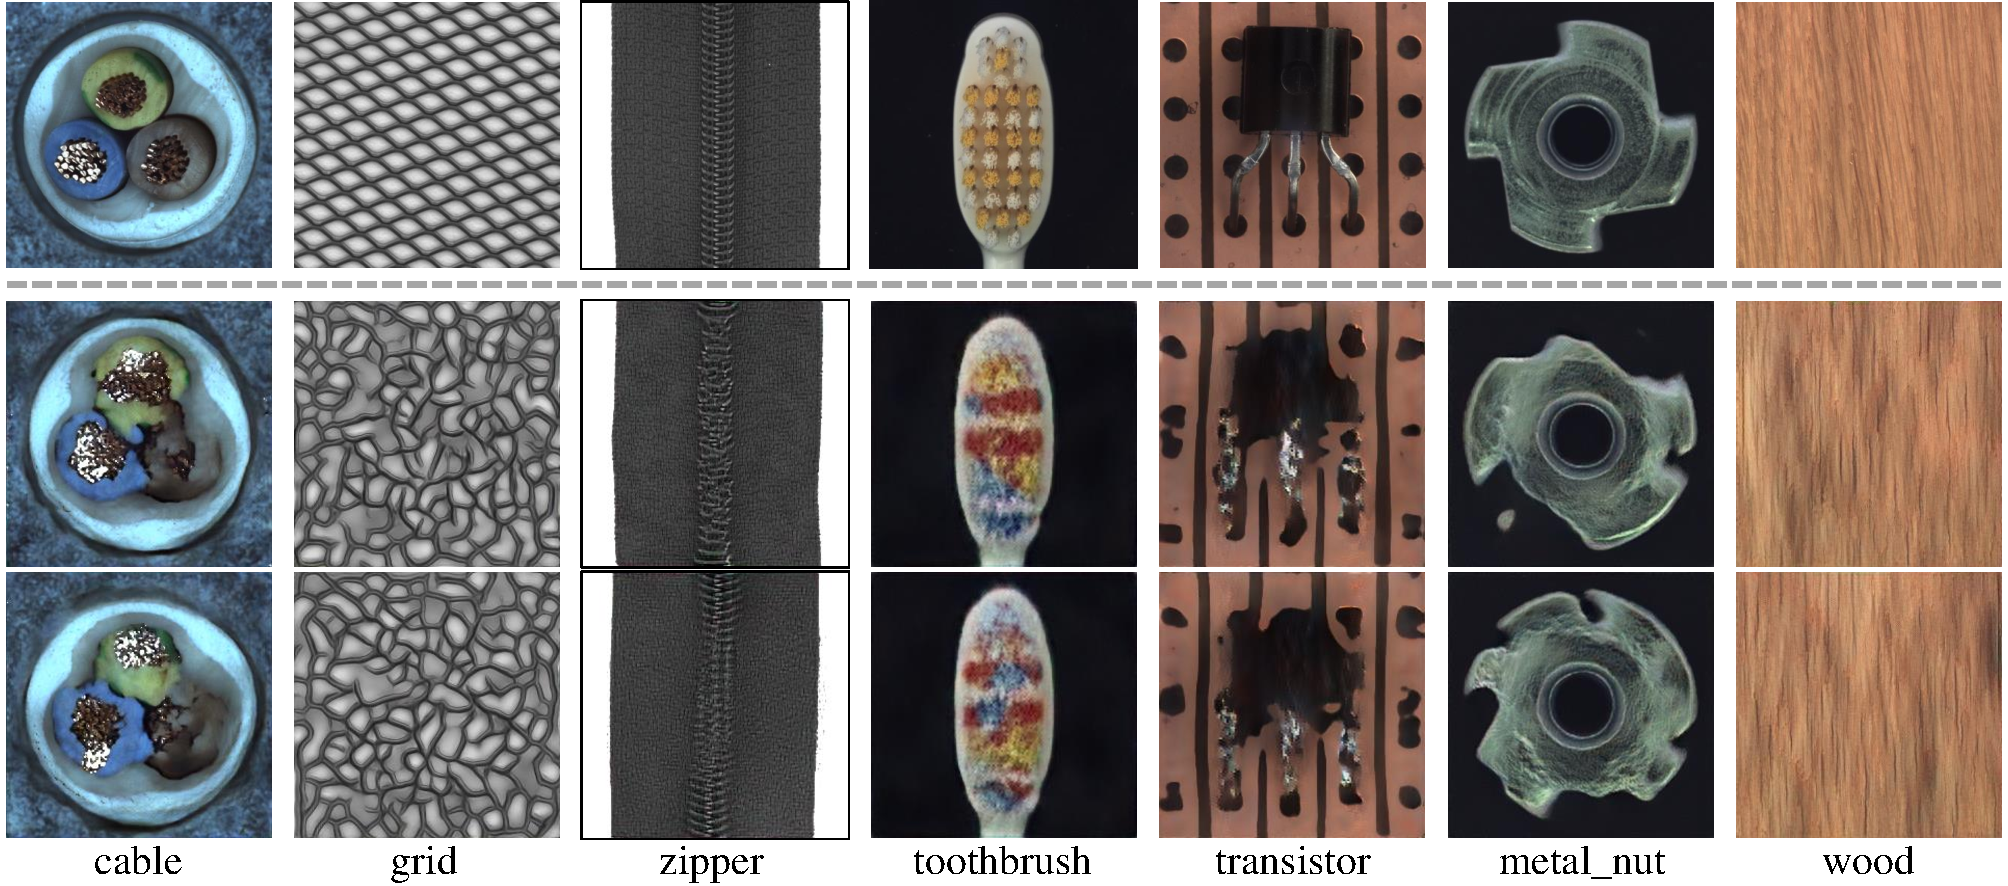
\includegraphics[width=0.7\linewidth]{images/mvtec_generation_results.pdf}
    \caption{Contrastive images generated by level-13 PatchDiff for MVTec AD~\cite{MVTecAD}. } 
    \label{fig: mvtec_generation}
\end{figure*}

\begin{table*}[!h]
    \centering
    % \footnotesize
    % \setlength{\belowcaptionskip}{0.2cm}
    % \setlength{\abovecaptionskip}{0.0cm}
    \renewcommand{\arraystretch}{1.2}
    \resizebox{\textwidth}{!}
    {
\begin{tabular}{cl|c|c|c|c|c|c|c|c}
\toprule
% \multicolumn{2}{c|}{Category} & \makecell[c]{IGD\\\tiny{\citealp{IGD}}} & \makecell[c]{PSVDD\\\tiny{\citealp{PSVDD}}} & \makecell[c]{FCDD\\\tiny{\citealp{FCDD}}} & \makecell[c]{CutPaste\\\tiny{\citealp{CutPaste}}} & \makecell[c]{NSA\\\tiny{\citealp{NSA}}} & \makecell[c]{DRAEM\\\tiny{\citealp{DRAEM}}} & \makecell[c]{DSR\\\tiny{\citealp{DSR}}} & \makecell[c]{GRAD\\\tiny{Ours}} \\ \midrule
\multicolumn{2}{c|}{Category}     & IGD & PSVDD & FCDD & CutPaste &NSA & DRAEM & DSR & GRAD \\ \midrule
\multirow{5}{*}{Texture} 
& carpet & (94.7, 82.8 ) & (92.9, 92.6) & (96.0, - ) & (93.1, 98.3) & (95.5, 95.6) & (95.5,97.0) & (-, \textbf{100.}) & (\textbf{96.5}, 98.2) \\
& grid & (97.7, 97.8 ) & (94.6, 100.) & (91.0, - ) & (\textbf{99.9}, 97.5) & (99.2, 99.9) & (99.7, 99.9) & (-, \textbf{100.}) & (97.2, \textbf{100.}) \\
& leather & (99.5, 95.8) & (90.9, 98.6) & (98.0, - ) & (\textbf{100.}, 99.5) & (99.5, 99.9) & (98.6, \textbf{100.}) & (-, \textbf{100.}) & (98.8, \textbf{100.}) \\
& tile & (78.0, 99.1) & (97.8, 91.4) & (91.0, - ) & (93.4, 90.5) & (\textbf{99.3}, \textbf{100.}) & (99.2, 99.6) & (-, \textbf{100.}) & (95.4, \textbf{100.}) \\
& wood & (89.1, 94.6) & (96.5, 90.8) & (88.0, - ) & (\textbf{98.6}, 95.5) & (90.7, 97.5) & (96.4, \textbf{99.1}) & (-, 96.3) & (87.2, 98.3) \\
\midrule
\multirow{10}{*}{Object} 
& bottle & (92.2, \textbf{100.}) & (98.6, 98.1) & (97.0, - ) & (98.3, 97.6) & (98.3, 97.7) & (\textbf{99.1}, 99.2) & (-, \textbf{100.}) & (96.5, \textbf{100.}) \\
& cable & (84.7, 90.6) & (90.3, 96.8) & (90.0, - ) & (80.6, 90.0) & (96.0, 94.5) & (94.7, 91.8) & (-, 93.8) & (\textbf{98.4}, \textbf{99.3}) \\
& capsule & (\textbf{97.7}, 91.5) & (76.7, 95.8) & (93.0, - ) & (96.2, 97.4) & (97.6, 95.2) & (94.3, \textbf{98.5}) & (-, 98.1) & (97.1, 96.4) \\
& hazelnut & (98.0, 99.7) & (92.0, 97.5) & (95.0, - ) & (97.3, 97.3) & (97.6, 94.7) & (\textbf{99.7}, \textbf{100.}) & (-, 95.6) & (96.6, 98.1) \\
& metal nut & (92.6, 91.3) & (94.0, 98.0) & (94.0, - ) & (99.3, 93.1) & (98.4, 98.7) & (\textbf{99.5}, 98.7) & (-, 98.5) & (93.7, \textbf{100.}) \\
& pill & (97.3, 87.3) & (86.1, 95.1) & (81.0, - ) & (92.4, 95.7) & (\textbf{98.5}, \textbf{99.2}) & (97.6, 98.9) & (-, 97.5) & (98.1, 95.7) \\
& screw & (97.0, 82.5) & (81.3, 95.7) & (86.0, - ) & (86.3, \textbf{96.7}) & (96.5, 90.2) & (97.6, 93.9) & (-, 96.2) & (\textbf{99.2}, 96.0) \\
& toothbrush & (97.7, 99.7) & (\textbf{100.}, 98.1) & (94.0, - ) & (98.3, 98.1) & (94.9, \textbf{100.}) & (98.1, \textbf{100.}) & (-, 99.7) & (98.0, 99.7) \\
& transistor & (84.4, 90.6) & (91.5, 97.0) & (88.0, - ) & (95.5, 93.0) & (88.0, 95.1) & (90.9, 93.1) & (-, 97.8) & (\textbf{97.8}, \textbf{100.}) \\
& zipper & (96.7, 97.0) & (97.9, 95.1) & (92.0, - ) & (\textbf{99.4}, 99.3) & (94.2, 99.8) & (98.9, \textbf{100.}) & (-, \textbf{100.}) & (98.3, 99.7) \\
\midrule
\multicolumn{2}{c|}{Average} & (93.1, 93.4) & (92.5, 93.2 ) & (92.1, 95.7) & (95.2, 96.0) & (96.3, 97.2) & (\textbf{97.3}, 98.0) & (-, 98.2) & (96.8, \textbf{98.7}) \\
\bottomrule
\end{tabular}}
\caption{Anomaly detection performance on MVTec AD dataset~\cite{MVTecAD}. Both pixel-level (left) and image-level (right) AUROC results are shown in each column. The best results are in bold.}
\label{tab: mvtec_main_detail}
\end{table*}

\subsection{Anomaly Detection and Localization}
In the main body, we exclusively present the averaged performance comparison on MVTec AD. In this section, we extend our analysis to provide a detailed result of the anomaly detection and localization performance across each individual sub-dataset within MVTec AD, and display anomaly maps on MVTec AD in Fig.~\ref{fig: main_mvtec_ad_results}. As shown in Table~\ref{tab: mvtec_main_detail}, we compare GRAD to IGD~\cite{IGD}, PSVDD~\cite{PSVDD}, FCDD~\cite{FCDD}, CutPaste~\cite{CutPaste}, NSA~\cite{NSA}, DRAEM~\cite{DRAEM}, and DSR~\cite{DSR}, all of which are independent of pretrained feature extractors. It is easy to find GRAD achieves a strong detection and localization of anomalies.  

\begin{figure*}[!h]
    \centering
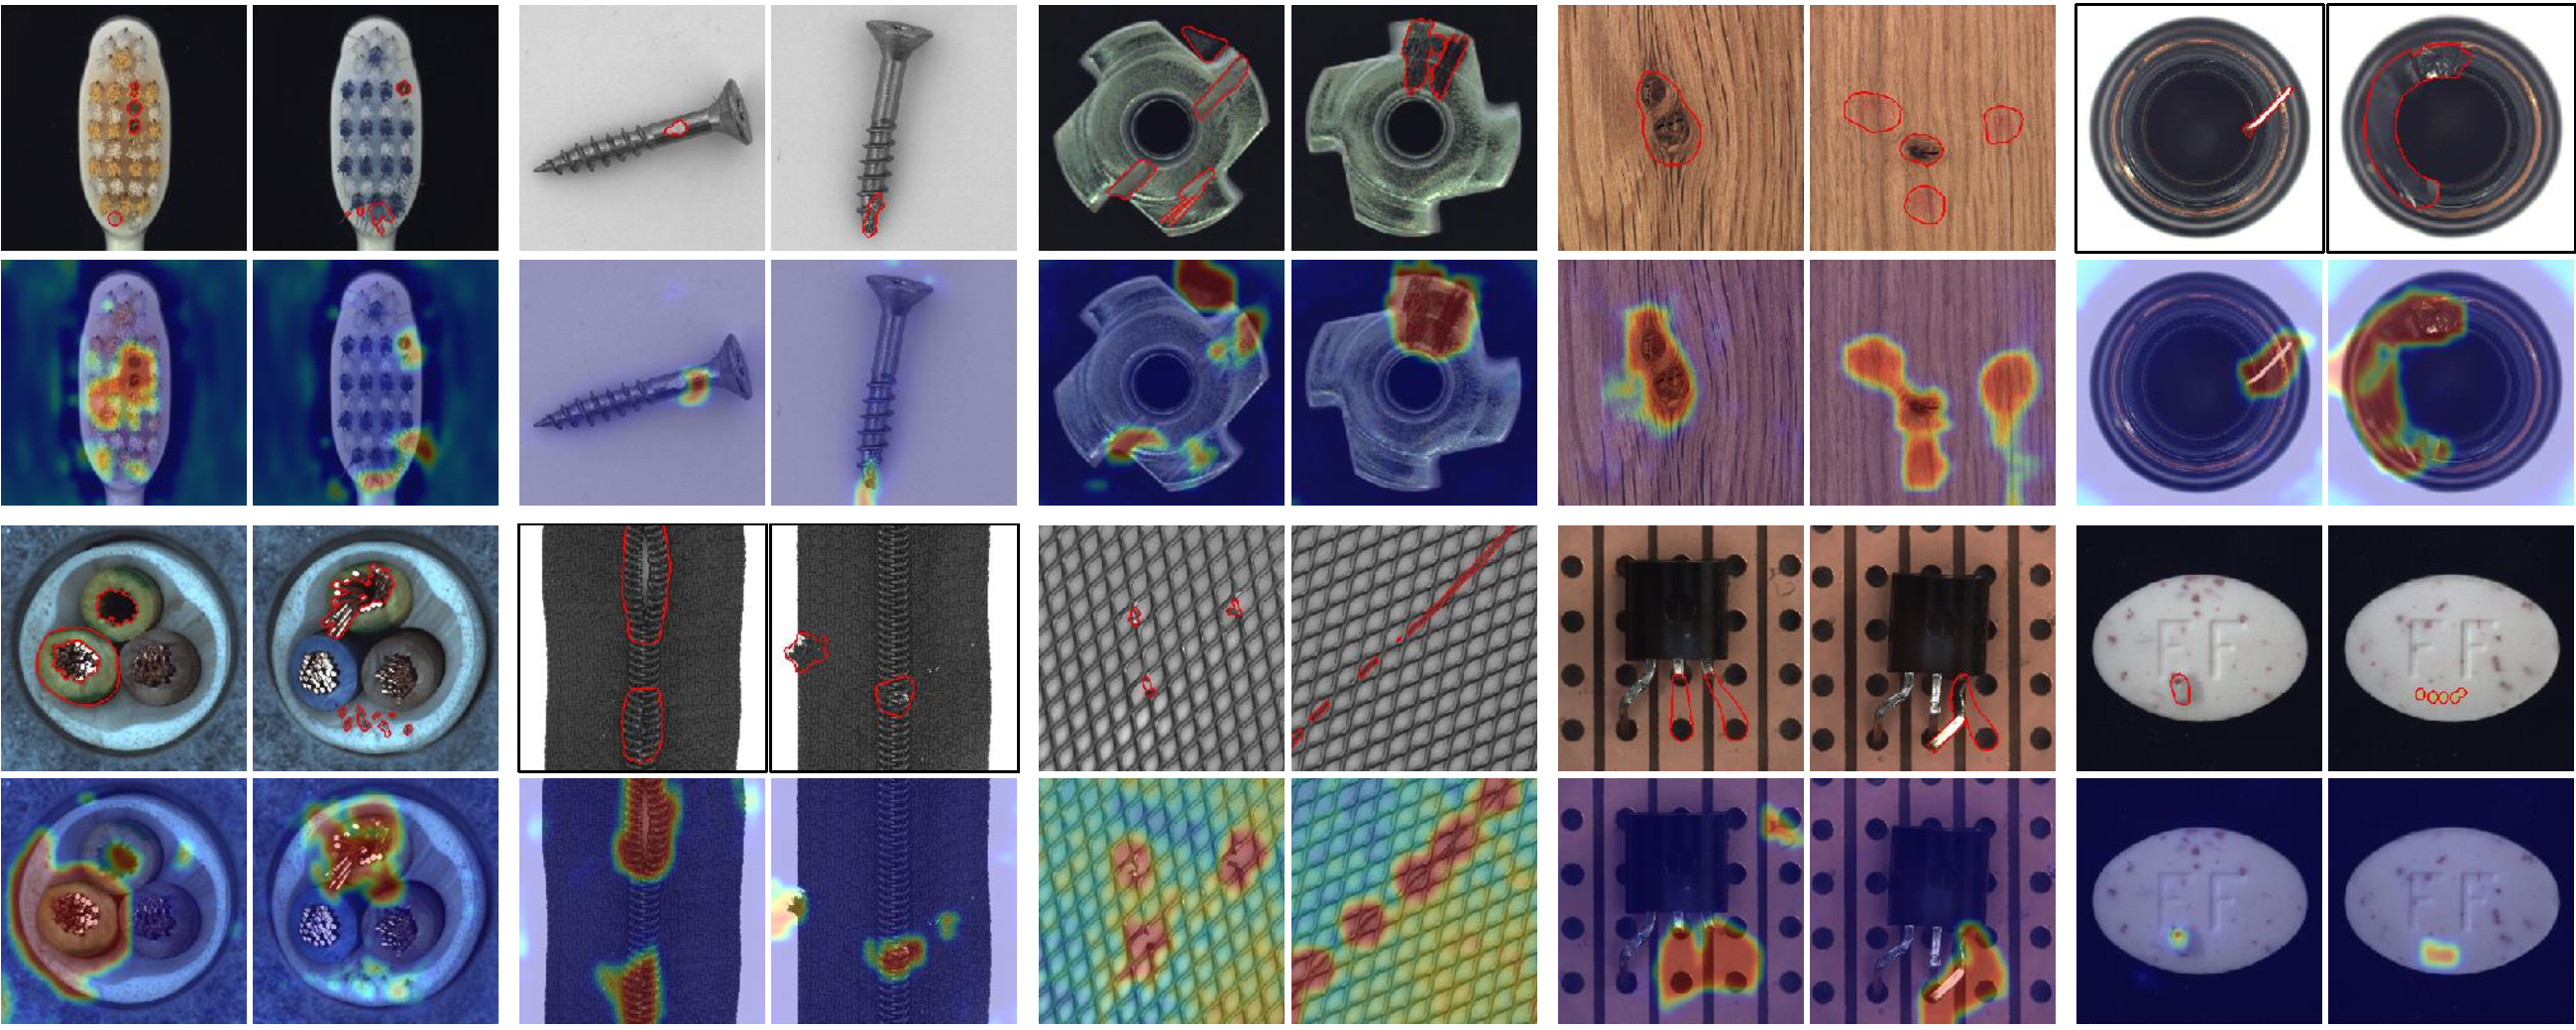
\includegraphics[width=0.9\linewidth]{images/mvtec_results.pdf}
    \caption{Defect localization results of GRAD on MVTec AD~\cite{MVTecAD}. } 
    \label{fig: main_mvtec_ad_results}
    % \vspace{-0.2cm}
\end{figure*}


% In addition, as shown in Table~\ref{tab:ablation_GRad_level}, we conduct an ablations study on selecting levels of patch-level detectors. It is easy to find that when integrating all three different levels of detectors, GRAD can achieve a strong performance for the detection of structural as well as logical anomalies.

% \begin{table}[!htbp]
% \centering
% \footnotesize
% \resizebox{0.3\textwidth}{!}{
% \begin{tabular}{ccc|c}
% \toprule
% \multicolumn{3}{c|}{Level Settings}& Image-level \\
% 136 & 68 & 34  & AUROC\\
% \midrule
% \checkmark &   \ding{55} & \ding{55}   &  85.2   \\
% \ding{55}& \checkmark & \ding{55} & 85.4 \\
% \ding{55}&\ding{55} & \checkmark & 75.1\\
% \checkmark & \checkmark & \ding{55}   &  86.8     \\ %
% \checkmark &   \ding{55} & \checkmark   &  86.4   \\
% \ding{55} & \checkmark & \checkmark  & 86.2 \\
% \checkmark & \checkmark & \checkmark &  \textbf{87.5}  \\
% \bottomrule
% \end{tabular}}
% \caption{Ablation study on detector levels. Detection AUROC results on MVTec LOCO dataset. The best results are in bold.}
% \label{tab:ablation_GRad_level}
% \end{table}



% \bibliography{aaai24}
% \bibliographystyle{aaai24}

% \end{document}


\section{Further Experiment Setup Details}
% \label{sec:experiment_details}
In this section, we will provide the more detailed experimental setup for the several applications in the main text. 
\subsection{Computational Resources}

For all numerical experiments in this paper, we use Python 3.9 with all algorithms implemented using \texttt{numpy} version 1.23.2. We run all experiments on a Linux machine with an Intel Xeon Silver 4114 CPU with 40 threads and 128GB of RAM. No GPU is used.

\subsection{APDAGD vs DE}
Each RGB image of size $32 \times 32 \times 3$ 
is transformed into grayscale, downscaled to $10 \times 10$, and flattened into a histogram of $100$ bins, all using the \texttt{scikit-image} library. 
We add $10^{-6}$ to every bin to avoid zeros. For every chosen pair of marginals, we divide each histogram by the maximum mass of the two, giving one marginal with a total mass of $1$ and other possibly less than $1$. For the cost matrix $\vC$, we use the squared Euclidean distance between pixel locations and normalize so $\norm{\vC}_\text{max} = 1$. The total transported mass is $0.8$ times the minimum total mass between the marginals. 

\subsection{Color Transfer}
% \label{sec:experiment_details_color_transfer}
Each RGB image can be considered a point cloud of pixels, and applying the color palette of one image into another is equivalent to applying the OT transport map to convert one color distribution to another. We choose the source image (Figure \ref{fig:color_transfer_comparison}a, \url{https://flic.kr/p/Lm6gFA}) and the target image (Figure \ref{fig:color_transfer_comparison}b, \url{https://flic.kr/p/c89LBU}) images, taken from Flickr. These images are chosen because they have quite distinct color palettes and different sizes. We follow the setup by \citep{Blondel-2018-Smooth} and implement the experiments as follows. Each image of size $h \times w \times 3$ is considered a collection of $hw$ pixels in 3 dimensions. Each image is quantized using $k$-means with $n = 100$ centroids. We apply $k$-means clustering to find $n$ centroids and assign to each pixel the centroid it is closest to. The image now becomes a color histogram with $n$ bins representing the centroids. For a pair of source and target images, similar to the previous subsection, we divide each histogram by the maximum total mass, yielding $\max\{\norm{\vr}_1, \norm{\vc}_1\} = 1$. Let $\va_1, \ldots, \va_n$ and $\vb_1, \ldots, \vb_n$ be the collections of centroids for the source and target images. The cost matrix is defined as $C_{i, j} = \norm{\va_i - \vb_j}_2^2$. With a partial transport map $\vX \in \RR_{+}^{n \times n}$, every centroid $\va_i$ in the source image is transformed to 
% $\hat{\va}_i = \dfrac{\sum_{j=1}^{n} X_{i, j} \vb_j}{\sum_{j=1}^{n} X_{i, j}}.$ 
$\hat{\va}_i = (\sum_{j=1}^{n} X_{i, j} \vb_j) / (\sum_{j=1}^{n} X_{i, j})$. All pixels in the source image previously assigned to $\va_i$ are now assigned to $\hat{\va}_i$. The total transported mass is set to $s = \alpha \min \{\norm{\vr}_1, \norm{\vc}_1\}$, where $\alpha \in [0, 1]$. To approximate the POT solution, we set $\varepsilon = 10^{-2}$ and run both Sinkhorn \cite{nhatho-mmpot} and APDAGD for 1,000 iterations. We set $\alpha = 0.1$, corresponding to transporting exactly 10\% of the allowed mass.
We plot the optimality gap $\inner{\vC}{\vX} - f^*$ for each transport map after every iteration in Figure \ref{fig:color_transfer_comparison} (c). As explained earlier, Sinkhorn with the accompanying rounding algorithm by \citep{altschuler2017near} does not produce a primal feasible solution, and its primal gap does not satisfy an error of $\varepsilon = 10^{-2}$ (indicated by the red line).

\subsection{Point Cloud Registration}
Previously, \cite{qin2022rigid} proposed a procedure to find such a transformation using partial optimal transport. Let the two marginal distributions be $\vr = \frac{1}{m} \ones_m$ and $\vc = \frac{1}{n} \ones_n$ and the cost matrix be $C_{i, j} = \norm{\vx_i - \vy_j}_2^2$. Given an optimal transport matrix $\vT \in \RR^{m \times n}$ between these marginals, the rotation matrix $\vR$ and translation vector $\vt$ are obtained by minimizing the energy: 
\begin{align*}
    \min_{\vR, \vt} ~ \sum_{i=1}^{m} \sum_{j=1}^{n} T_{i, j} \norm{\vx_i - (\vR \vy_j + \vt)}_2^2.
\end{align*}
This problem admits the closed-form solution
\begin{align*}
    \vR = \mathbf{V} \vS \mathbf{U}^\top, \quad \vt = \vu_x - \vR \vu_y,
\end{align*}
where $\vu_x = \frac{1}{m} \sum_{i=1}^{m} \vx_i$, $\vu_y = \frac{1}{n} \sum_{j=1}^{n} \vy_j$. The matrices $\mathbf{U}$, $\vS$ and $\mathbf{V}$ are obtained as follows. Let $\hat{\vX} \in \RR^{m \times 3}$ whose $i$th row is $(\vx_i - \vu_x)^\top$. Similar for $\hat{\vY} \in \RR^{n \times 3}$. Then, obtain the singular value decomposition of the matrix $\hat{\vX} \vT^\top \hat{\vX}^\top$ as $\mathbf{U} \mathbf{\Lambda} \mathbf{V}^\top$. Finally, $\vS = \diag(1, 1, \det(\mathbf{V} \mathbf{U}^\top))$.

To find the the matrix $\vT$, we follow the iterative procedure in \cite[Algorithm 1]{qin2022rigid} in which the point cloud $Q$ is updated gradually until convergence. In our implementation, we set the initial value for $\gamma$ (strength of entropic regularization) to 0.004 and the annealing rate of $\gamma$ to $\lambda = 0.99$. With each $\gamma$, we find the OT matrix using Sinkhorn, and the POT matrix using two methods: Sinkhorn and APDAGD. The iterative process ends when the change of $\vR$ in Frobenius norm falls below $10^{-6}$.
\section{Further Numerical Experiments}
% \label{appn:experiments}

\subsection{Run Time for Varying $\varepsilon$}
\begin{figure}
    \centering
    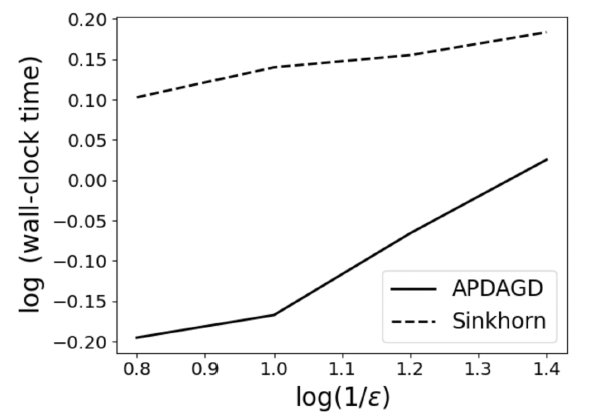
\includegraphics[width=0.5\linewidth]{figs/runtime_vary_eps.png}
    \caption{Comparison of wall-clock running time between APDAGD and Sinkhorn for varying $\varepsilon$}
    \label{fig:runtime_for_varying_epsilon}
\end{figure}
With the similar setting to Figure \ref{fig:de_vs_apdagd} of using images in the CIFAR-10 dataset, we provide additional experiments showcasing that APDAGD is better than Sinkhorn in wall-clock time in terms of both aggregate run time cost in Figure \ref{fig:runtime_for_varying_epsilon}. Moreover, for aggregate wall-clock time, we note that previous works showed that gradient methods and especially APDAGD are practically faster than Sinkhorn \cite[Figure 1]{Dvurechensky-2018-Computational}. This claim is further supported by Figure \ref{fig:runtime_for_varying_epsilon} since it reproduce the results from \cite[Figure 1]{Dvurechensky-2018-Computational} which compare the runtime of Sinkhorn and APDAGD in the context of OT. 
\subsection{Revised Sinkhorn}
We again utilize the same setting Figure \ref{fig:de_vs_apdagd} and Run Time for Varying $\varepsilon$ with CIFAR-10 dataset. On the left, we empirically verify our theoretical bounds in Theorem \ref{contraint_violation}, by showing that increasing $A$ potentially lead to a better feasibility of Sinkhorn. For the figure on the right, we show that the increase of $A$ to a sufficient size can lead to more number of iterations to convergence of Sinkhorn. This is also suggested by the worsened theoretical complexity of revised Sinkhorn (Theorem \ref{them:revised_sinkhorn_complexity}).
\begin{figure}
    \centering
    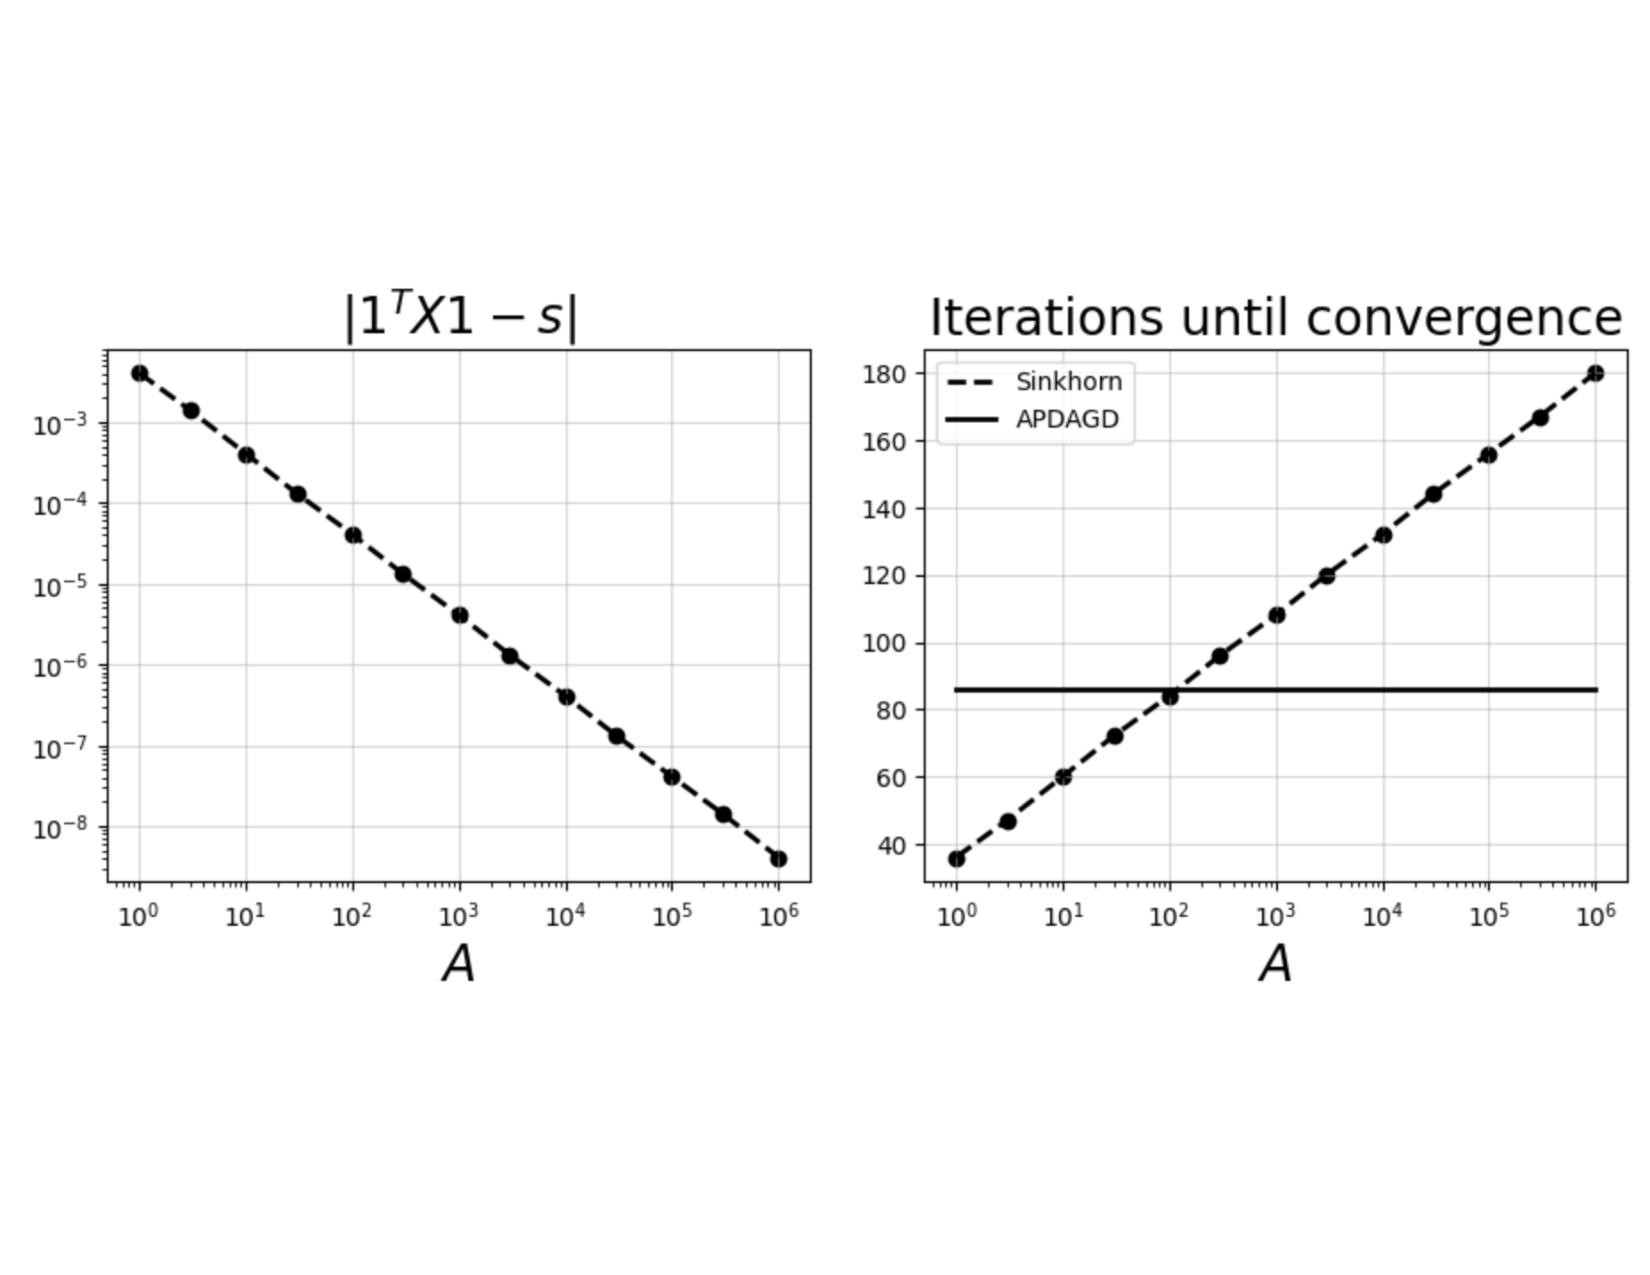
\includegraphics[width=0.8\linewidth]{figs/revised_sinkhorn.pdf}
    \caption{Left: Sinkhorn constraint violation with respect to $A$. Right: Number of iterations for both APDAGD and Sinkhorn until a pre-defined suboptimality is achieved.}
    \label{fig:revised_sinkhorn}
\end{figure}

\subsection{Domain Adaptation}
In our setting, the source and target datasets contain different numbers of data points ($N_s = 300$ and $N_t = 400$, respectively). For OT, we use Sinkhorn to approximate the OT matrix of size 300 $\times$ 400, then transform the source examples according to Courty et al. (2017). For POT, we use K-means clustering to transform the target domains to a histogram of $300$ bins. The two unbalanced marginals are then normalized so that $\left\| r \right\|_1 = 0.75, \left\| c \right\|_1 = 1.0$, and we set $s = 0.999 \times \min\{ \left\| r \right\|_1, \left\| c \right\|_1 \}$ then use APDAGD to find the POT matrix between these two unbalanced marginals. The source examples are transformed similarly. Finally, for both methods (OT and POT), we train a support vector machine with the radial basis kernel (parameter $\sigma^2 = 1$) using the transformed source domain. In the Figure \ref{fig:POT_vs_OT} we report the accuracy on the target domain using 20,000 test examples. All hyperparameters are set to be equal.


Here we implement and compare Domain Adaptation with OT to Domain Adaptation with POT, which is calculated with two different algorithms Sinkhorn (infeasible rounding) and APDAGD (with our novel \textsc{Round-POT}). In \citep{courty2017joint}, the authors presented an OT-based method to transform a source domain to a reference target domain such that the their densities are approximately equal. We present a binary classification setting involving the "moons" dataset. The source dataset is displayed as colored scatter points. The target dataset comes from the same distribution, but the points go to a rotation of 60 degrees (black scatter points), representing a domain covariate shift. Additional experimental details are further described in Further Experiments Setup Details section in Appendix. % We then use APDAGD to find the POT matrix between these two unbalanced marginals. The source examples are transformed similarly. Finally, for both methods (OT and POT), we train a support vector machine with the radial basis kernel (parameter $\sigma^2 = 1$) using the transformed source domain. 
To summarize the results, POT offers much more practicality as it does not require normalizing both marginals to have a sum of 1 in contrast to OT. More importantly, POT avoids bad matchings to outliers due to the flexibility in choosing the amount of mass transported, resulting in a higher accuracy than OT. Furthermore, linking back to Remark \ref{remark:violation}, the infeasibility Sinkhorn degrades the practical performance of POT for Domain Adaption and consequently leads to a worse accuracy compared APDAGD. This is because the optimal mapping between the source and target domains requires the exact fraction of mass to be transported which APDAGD fulfills practically in contrast to Sinkhorn.  

\begin{figure}
    \centering
    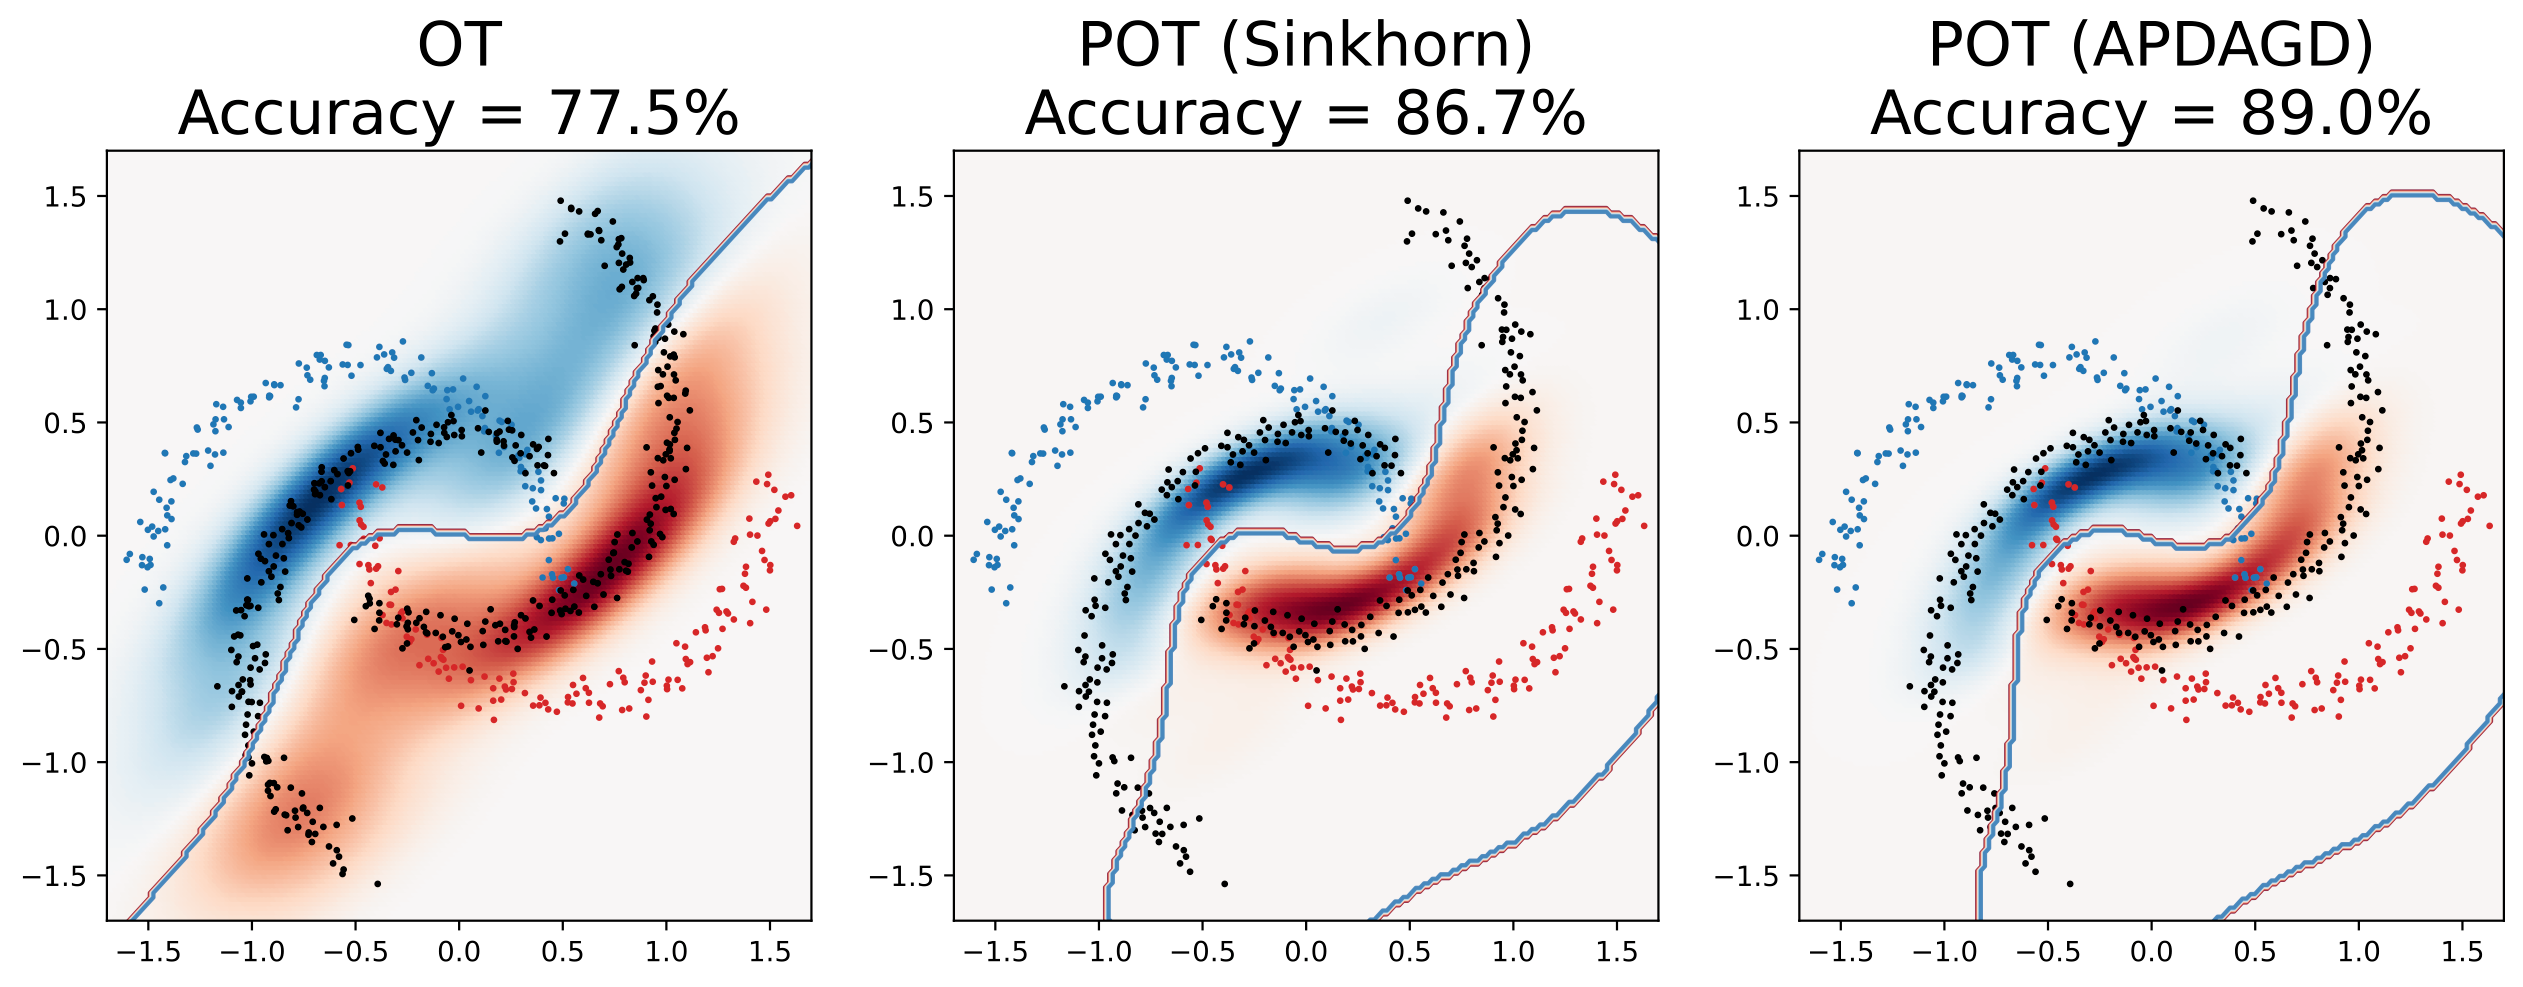
\includegraphics[width=1\linewidth]{figs/POT_vs_OT.png}
    \caption{Domain adaptation with OT and with POT. POT offers a flexibility in choosing the mass transported and helps avoid the need to normalize both marginals to have a sum of $1$, resulting in better complexity than OT. APDAGD demonstrates better accuracy in the novel domain than Sinkhorn, which suffers from infeasibility.}
    \label{fig:POT_vs_OT}
\end{figure}

\subsection{Synthetic Data}
\begin{figure}[ht]
    \centering
    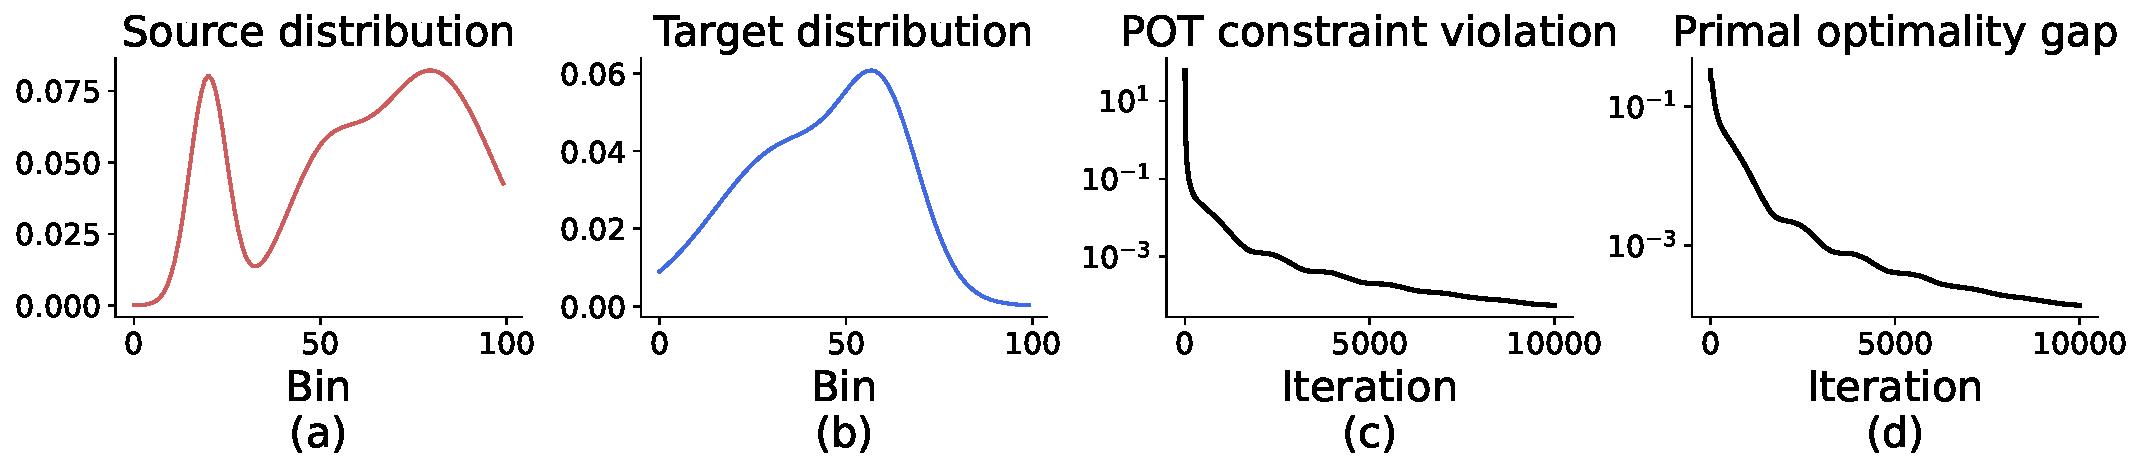
\includegraphics[width=1\linewidth]{figs/apdagd_synthetic.pdf}
    \caption{Convergence of APDAGD on a synthetic setting.}
    \label{fig:apdagd_synthetic}
\end{figure}

In this section we design a POT setting and evaluate the convergence of APDAGD. The two marginals are unnormalized Gaussian mixtures. We then discretize them into histograms of $n = 100$ bins each and perform normalization so that $\norm{\vr}_1 = 5$, $\norm{\vc}_1 = 3$. The total transported mass is set to $s = 0.9 \min\{ \norm{\vr}_1, \norm{\vc}_1 \} = 2.7$, and the cost matrix represents squared Euclidean distances between every pair of bins in the source and target histograms. In other words, $C_{i, j} = (i - j)^2$ for all $i, j = 1, \ldots, n$. Finally, we divide $\vC$ by its maximum entry to have $\norm{\vC}_\text{max} = 1$.

We use \texttt{cvxpy} with the GUROBI backend to solve the linear problem \eqref{prob:pot_with_pq}, and denote by $f^*$ the optimal objective value. This will be used to calculate the primal optimality gap.

The approximate POT solution is solved using APDAGD, where we set the additive suboptimality error $\varepsilon$ to $10^{-3}$. We run APDAGD for 10,000 iterations and keep track of two errors. The first error is constraint violation, equal to $\norm{\vX \ones + \vp - \vr}_1 + \norm{\vX^\top \ones + \vq - \vc}_1 + \lvert \ones^\top \vX \ones - s \rvert$ where $\vX$, $\vp$ and $\vq$ are part of the solution $\vx_k$ found after each iteration. The second error is the optimality gap for the primal objective. To calculate this, we need to round the solution so that it becomes primal feasible. We use our rounding algorithm described in Rounding Algorithm Section to round $\vX$, $\vp$, and $\vq$ after each iteration, giving us $\bar{\vX}$, $\bar{\vp}$ and $\bar{\vq}$. The primal gap then is $\inner{\vC}{\bar{\vX}} - f^*$.

% \subsection{Extra Details for Domain Adaptation}
% Here we provide a new experimental result in domain adaptation. In Courty et al. (2017), the authors presented an OT-based method to transform a source domain to a reference target domain such that the their densities are approximately equal. We present a binary classification setting involving the "moons" dataset. The source dataset is displayed as colored scatter points. The target dataset comes from the same distribution, but the points go to a rotation of 60 degrees (black scatter points below), representing a domain covariate shift.

% In our setting, the source and target datasets contain different numbers of data points ($N_s = 300$ and $N_t = 400$, respectively). For OT, we use Sinkhorn to approximate the OT matrix of size 300 $\times$ 400, then transform the source examples according to Courty et al. (2017). For POT, we use K-means clustering to transform the target domains to a histogram of $300$ bins. The two unbalanced marginals are then normalized so that $\left\| r \right\|_1 = 0.75, \left\| c \right\|_1 = 1.0$, and we set $s = 0.999 \times \min\{ \left\| r \right\|_1, \left\| c \right\|_1 \}$ then use APDAGD to find the POT matrix between these two unbalanced marginals. The source examples are transformed similarly. Finally, for both methods (OT and POT), we train a support vector machine with the radial basis kernel (parameter $\sigma^2 = 1$) using the transformed source domain. In the figure below we report the accuracy on the target domain using 20,000 test examples. POT offers a flexibility in choosing the mass transported and helps avoid the need to normalize both marginals to have a sum of $1$. POT also results in a higher accuracy than OT.

% \begin{figure}
%     \centering
%     \includegraphics[width=1\linewidth]{figs/POT vs OT.png}
%     \caption{Domain Adaptation with OT vs with POT}
%     \label{fig:POT_vs_OT}
% \end{figure}

% In figure \ref{fig:Sinkhorn_vs_APDAGD}, we additionally compare two methods of approximating the POT matrix in this paper: Sinkhorn (which outputs a primal infeasible solution) and APDAGD. All hyperparameters are equal. The results indicate that, in addition to giving a primal feasible solution, APDAGD gives a higher accuracy than Sinkhorn.  
% % \begin{figure}
% %     \centering
% %     \includegraphics[width=1\linewidth]{figs/Sinkhorn vs APDAGD.png}
% %     \caption{Domain Adaptation by APDAGD vs by Sinkhorn}
% %     \label{fig:Sinkhorn_vs_APDAGD}
% % \end{figure}

\subsection{Scalability of APDAGD}
Given the complexity claims in the paper, it is important to show how running time scales with $n$, the number of supports in each marginal. In the below Figure \ref{fig:scalability}, we show the wall-clock time of running APDAGD to solve the POT problem between two Gaussian mixtures (shown in the end of the appendix). We fix the error tolerance to $\varepsilon = 10^{-1}$ and vary $n$ in the set $\{ 10, 30, 100, 300, 1000, 3000, 10000 \}$. The figure plots wall-clock time in seconds against $n$. The expected slope of the best-fit line between $\log(\text{time})$ and $\log(n)$ should be at most 2.5, as the complexity is $\widetilde{O}(n^{2.5} / \varepsilon)$. We find that the slope is $2.19$, which is consistent with the upper bound. Furthermore, the correlation is statistically significant.

\begin{figure}
    \centering
    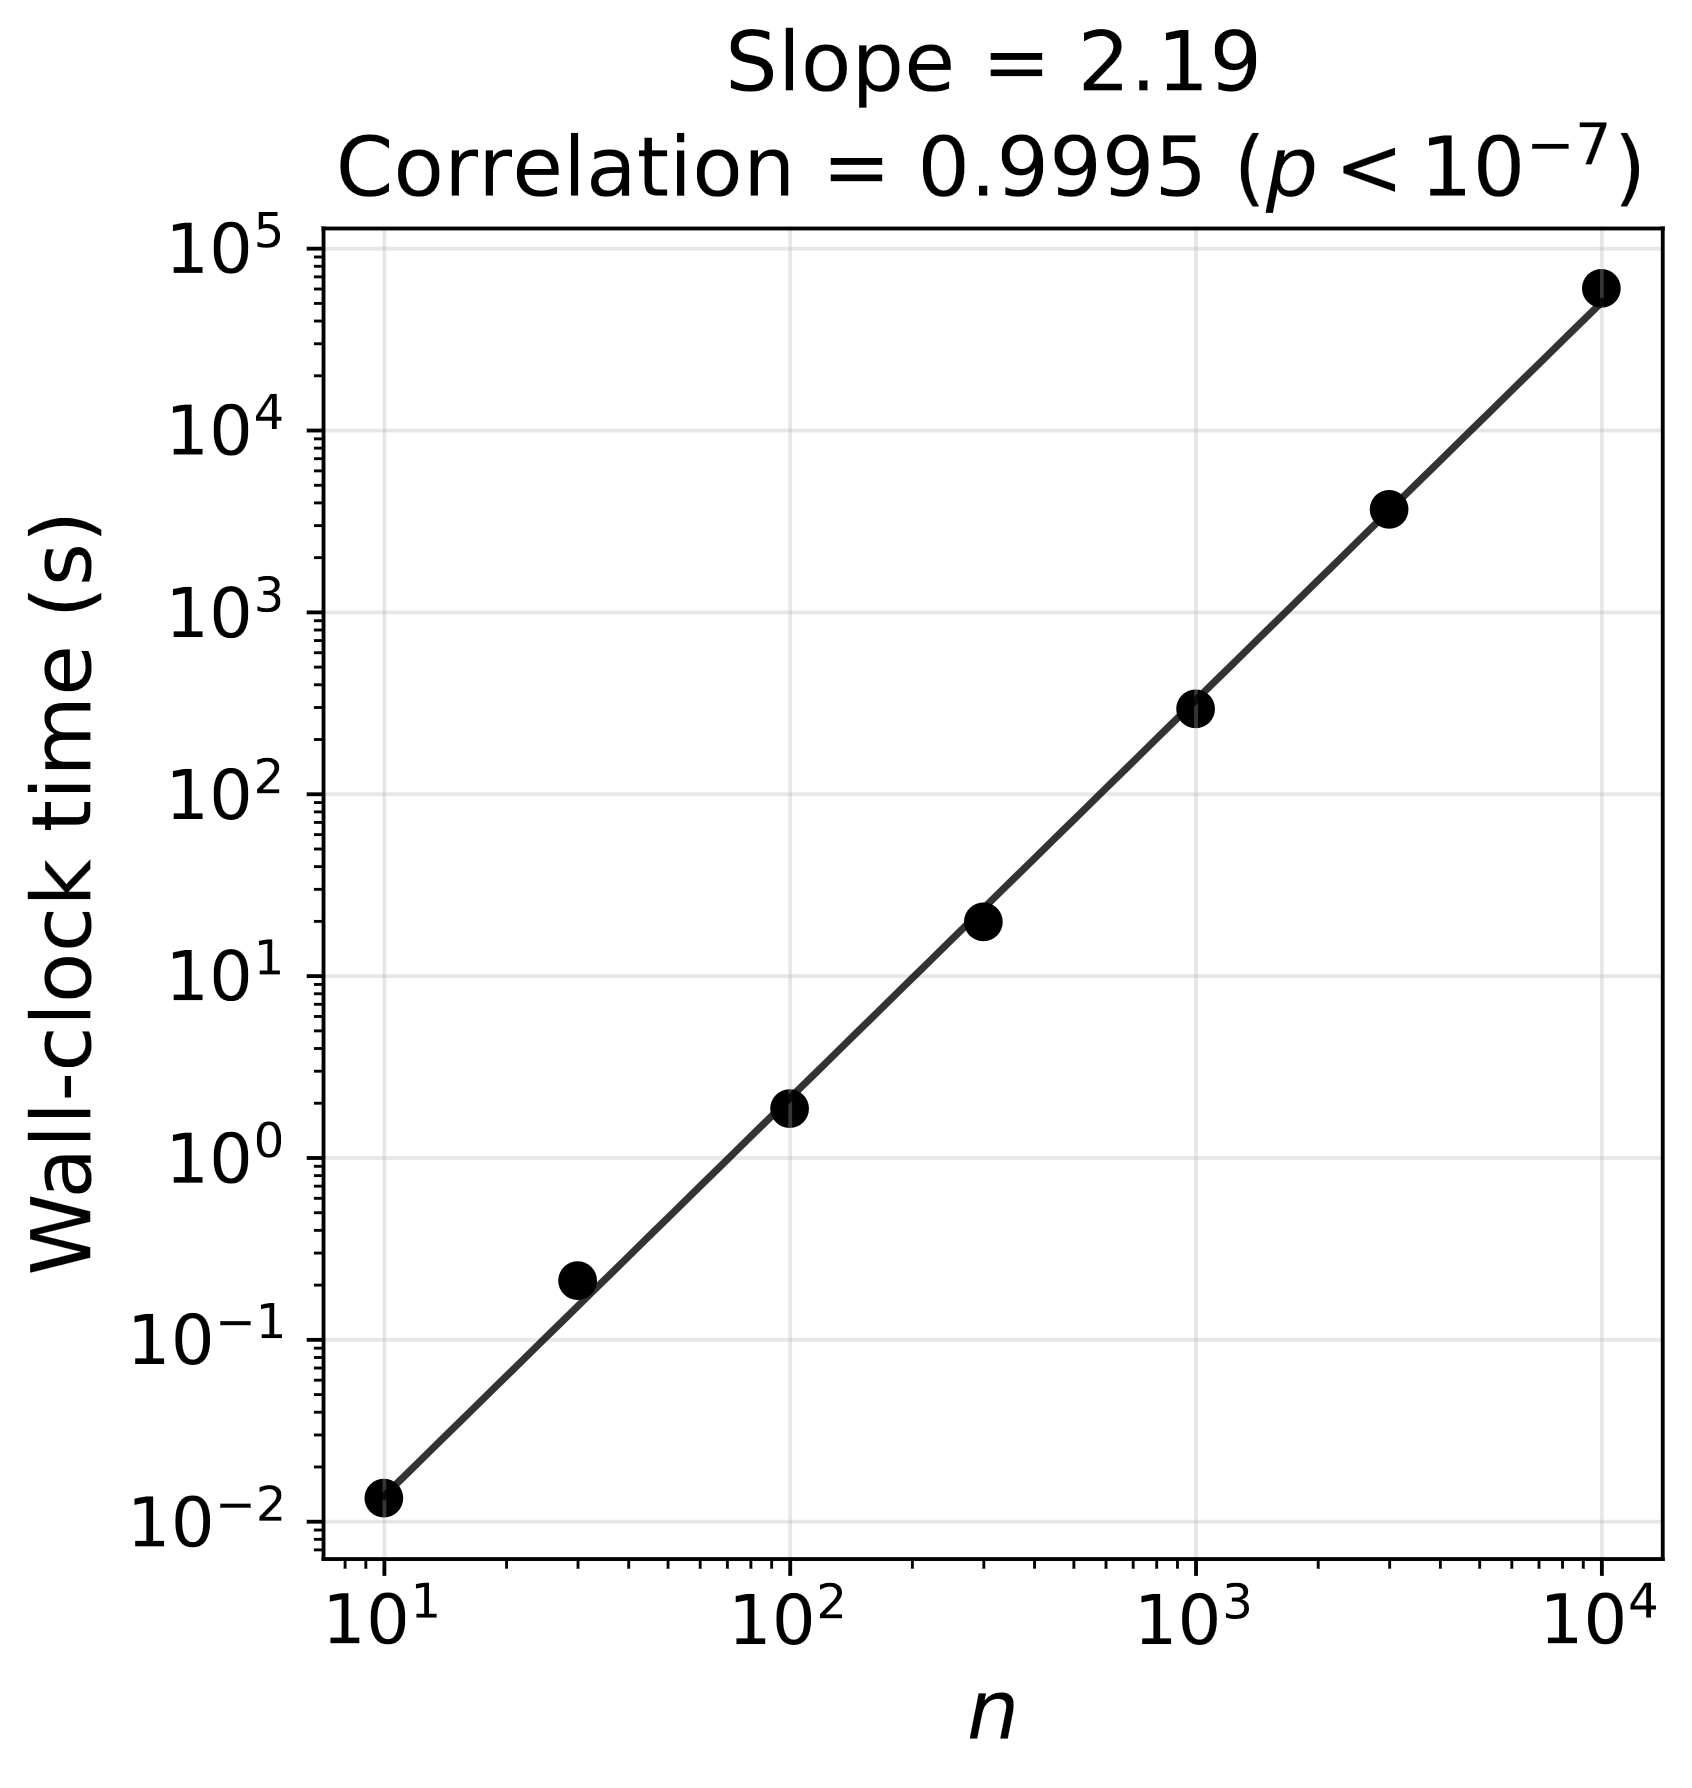
\includegraphics[width=0.4\linewidth]{figs/scalability.png}
    \caption{Wall-clock time of solving POT with APDAGD against $n$}
    \label{fig:scalability}
\end{figure}

\newpage




\end{document}
